\documentclass[11pt,a4paper]{article}
\usepackage{a4,graphicx,color}
\usepackage{footnpag,array}
\usepackage{fancyhdr,fancybox}
\usepackage{amsmath}
\usepackage{epsfig}
%\usepackage{french}
% Ca fait chier de pas pouvoir utiliser ca : les captions ne sont plus en italique et ca marque "Figure 1:" [sans espace devant le chiffre] au lieu de "{\sc Fig.} 1 :". 'faut que je me redefinisse une commande "caption".

\oddsidemargin=-7mm
\textwidth=174mm
\addtolength{\headheight}{0.55cm}
\makeatletter
\def\@captype{figure}
\makeatother

\newenvironment{changemargin}[2]{\begin{list}{}{
\setlength{\topsep}{0pt}
\setlength{\leftmargin}{0pt}
\setlength{\rightmargin}{0pt}
\setlength{\listparindent}{\parindent}
\setlength{\itemindent}{\parindent}
\setlength{\parsep}{0pt plus 1pt}
\addtolength{\leftmargin}{#1}
\addtolength{\rightmargin}{#2}
}\item }{\end{list}}
\newcommand{\itemb}[1]{\setlength{\parindent}{-1cm}\begin{changemargin}{1cm}{0cm}#1\end{changemargin}\setlength{\parindent}{0cm}}

% Profondeur de \subsubsection = 3
\setcounter{tocdepth}{3}     % Dans la table des matieres
\setcounter{secnumdepth}{3}  % Avec un numero.

\begin{document}

\pagestyle{fancy}
\renewcommand{\sectionmark}[1]{\markboth{#1}{}}
\lhead{V0Finder and XiFinder}
\rhead{\thesection\ - {\em \leftmark}}
%\renewcommand{\caption}[1]{\addtocounter{figure}{1}Figgg \thefigure : {#1}}  %Evidemment, ca n'est pas considere comme un caption ! Donc pour lui c;est juste du texte qu'il ajoute apres chaque figure (=> pas a la ligne, pas centre, et apparait pas dans la table des matieres).
\def\figurename{{\sc Fig.}} %C'est mieux, mais j'ai toujours pas d'espace entre le chiffre et les ":". C'est chose faite avec le truc qui suit :-))
\makeatletter
\renewcommand{\fnum@figure}{\figurename~\thefigure~}
\makeatother
%Reste le probleme du texte qui n'est pas automatiquement en italique.
%\newcommand{\mycaption}{\caption}
%\renewcommand{\caption}[1]{\mycaption{#1}}
%Ca va pas, c'est malheureusement recursif. Tant pis, je me redefinis un caption perso.
\newcommand{\mycaption}[1]{\caption[\hspace{-10pt}{#1}]{{\em {#1}.}}}
\newcommand{\mycaptionBis}[2]{\caption[\hspace{-10pt}{#1}]{{\em {#2}.}}}
% Et j'en ai profite pour raccourcir l'espace dans la liste des figures (entre le numero et la legende), et pour gerer le point correctement (pas de point dans la liste des figures, mais un point a la fin des legendes sous les figures). Youpi, c'est cool LaTeX !  :-D

%\discretionary{Avant la coupure}{apr�s}{s'il n'y en a pas}
%\discretionary{}{-}{}
%


%\newenvironment{maliste}
%{ \begin{list}
%        {$\bullet$}
%        {\setlength{\labelwidth}{30pt}
%         \setlength{\leftmargin}{35pt}
%         \setlength{\itemsep}{\parsep}}}
%{ \end{list} }
% Si on remplace itemsep par un nombre avec ou sans unite : ca chie.
% Si on remplace a la fois parsep  et itemsep : ca compile, mais aucun resultat (ca printe les valeurs sur le document, en fait).

\newenvironment{maliste}
{\vspace{-7pt}
 \begin{list}
 {$\bullet$}
 {\setlength{\labelwidth}{30pt}
 \setlength{\leftmargin}{35pt}
 \setlength{\itemsep}{-4pt}}}
{\end{list}
 \vspace{-6pt}}






%\parindent40pt
%
%\begin{center}
%
%~
%
%\thispagestyle{empty}
%
%\vspace{8cm}
%
%{\Huge\bf XiFinder and V0Finder documentation}
%
%\end{center}

%\begin{picture}(21cm,29.7cm)(0cm,0cm)
%\put(5cm,5cm){\circle(3cm)}
%\end{picture}

\thispagestyle{empty}
\unitlength 1mm
\begin{picture}(200,220)(20,10)
%\put(5,0){\vector(1,0){190}}
%\put(5,0){\vector(0,1){230}}
\linethickness{1mm}
%\put(5,0){\framebox(190,250)
%{\vspace{2cm}\\
%{\Huge\bf XiFinder and V0Finder documentation}\\
%\vspace{1cm}\\
%{\tt StRoot/StSecondaryVertexMaker/}\\
%\vspace{1cm}\\
%\hfill {\small --- Julien Faivre}}
%}
%Ca marche pas, ca met rien a la ligne ; laisser une ligne vide non plus.
%\put(5,0){\framebox(190,250){~\vspace{-3cm}\Huge\bf XiFinder and V0Finder documentation}}
%Marche pas du tout...
\put(5,0){\framebox(190,250){}}
\linethickness{1pt}
\put(6,1){\framebox(188,248){}}
\put(5,165){\makebox(190,50){\Huge\bf Secondary vertex Finders documentation}}
\put(40,140){\makebox(100,50)[l]{\Large\tt StRoot/StSecondaryVertexMaker/ :}}
\put(70,135){\makebox(100,50)[l]{\large\tt StV0FinderMaker.cxx}}
\put(70,130){\makebox(100,50)[l]{\large\tt StV0FinderMaker.h}}
\put(70,125){\makebox(100,50)[l]{\large\tt StXiFinderMaker.cxx}}
\put(70,120){\makebox(100,50)[l]{\large\tt StXiFinderMaker.h}}
\put(70,115){\makebox(100,50)[l]{\large\tt StKinkMaker.cxx}}
\put(70,110){\makebox(100,50)[l]{\large\tt StKinkMaker.h}}
\put(70,105){\makebox(100,50)[l]{\large\tt StKinkLocalTrack.cc}}
\put(70,100){\makebox(100,50)[l]{\large\tt StKinkLocalTrack.hh}}
\put(40,90){\makebox(100,50)[l]{\Large\tt StRoot/StSecondaryVertexMaker/doc/ :}}
\put(70,85){\makebox(100,50)[l]{\large\tt docXiFinder.tex}}

%\put(5,50){\makebox(190,50){\hfill --- Julien Faivre\hspace{40pt}}}
%\put(5,45){\makebox(190,50){\hfill Strangeness group\hspace{40pt}}}
%\put(5,40){\makebox(190,50){\tt\small\hfill julien.faivre@ires.in2p3.fr\hspace{40pt}}}

\put(5,52){\makebox(160,50){\bf\hfill -- Strangeness group -- \hspace{40pt}}} %Prend ni \em, ni \it ! (Change rien).
\put(5,46){\makebox(155,50){\hfill People to contact : \hspace{40pt}}}
\put(5,30){\makebox(190,50){
\hfill
\begin{tabular}{|r@{ --- }l|}
\hline
Betty Bezverkhny & {\sc SVT} \\ %Tiens, il prend pas non plus \sc, en fait...
Gene van Buren & V0Finder \\
Helen Caines & {\sc SVT} \\
Julien Faivre & V0Finder and XiFinder \\
Camelia Mironov & KinkFinder \\
\hline
\end{tabular}
\hspace{40pt}
}}

\put(5,12){\makebox(190,50){\small\hfill (Up-to-date e-mail adresses can be taken from the hypernews).\hspace{27pt}}}
\end{picture}







\newpage


\section*{}
\addcontentsline{toc}{section}{Table of contents}
\vspace{-2.5cm}
\tableofcontents

\thispagestyle{empty}




\newpage



\section*{}
\addcontentsline{toc}{section}{List of figures}
\listoffigures

\thispagestyle{empty}


\newpage



\setlength{\parindent}{50pt}

\section{What are the V0Finder and XiFinder ?}

Let's first define the 3 different sorts of secondary vertices :
\begin{itemize}
\item Kink vertices : when a charged particle decays into a charged plus a neutral,
\item V0 vertices : when a neutral particle decays into two charged particles,
\item Xi vertices : when a charged particle decays into a charged plus a neutral, and then the neutral daughter decays itself into two charged particles. One can't say that a Xi vertex is a Kink followed by a V0, because both charged tracks (mother and daughter) have to be seen in the {\sc tpc} in order to say that the vertex is a kink. This is not the case for Xi vertices, because the $c\tau$ of particles that do a Xi vertex is much shorter than the distance between the primary vertex and the {\sc tpc} ($50~cm$), even shorter than the distance to the first layer of the {\sc svt} ($6.7~cm$, versus $c\tau_{_\Xi} = 4.9~cm$ and $c\tau_{_\Omega} = 2.5~cm$).
%c\tau__\Xi marche mais fait erreurs a la compilation.
\end{itemize}

People working on strange particles in the strangeness group need a piece of code that is able to reconstruct the primary strange particles from the tracks. Those strange particles can be divided into two groups~:
\begin{itemize}
\item {\bf V0's :} those particles ($\Lambda$, $K^0_s$) decay into two particles ($\Lambda \longrightarrow p \pi^-$, $K^0_s \longrightarrow \pi^+ \pi^-$). We need to be able to search and find them using only the daughters' tracks (that's all we have !).
\item {\bf Xi's :} those particles ($\Xi$, $\Omega$) decay into 1 charged particle -- called bachelor -- and a $\Lambda$ ($\Xi \longrightarrow \Lambda \pi^-$, $\Omega \longrightarrow \Lambda K^-$). The $\Lambda$, as said in the previous item, decays into two particles. So here, we need to find all combinations of 3 charged particles that are possibly the daughters of a unique strange particle.
\end{itemize}
The algorithms of those codes are described in section \ref{sec3}.

From the beginning of {\sc star} and until year 2002, the codes used were what will be called in this documentation {\em exiam} and {\em ev0am}. They are Fortran codes, located in {\tt pams/global/exi/\-exiam.F} and {\tt pams/global/\-ev0/\-ev0\_am2.F}, with other files that are necessary for the code to be run (basically subroutines and interfacing functions).

So here is the ``old" way to do things : the {\sc bfc} is run, and it calls the series of makers that it is supposed to call. Among those makers are {\tt StXiMaker} and {\tt StV0Maker} -- the strangeness makers, with {\tt StKinkMaker} -- and they are run after nearly all the other makers of the {\sc bfc}, since they need the tracks to be reconstructed and the primary vertex to be found. The V0Maker is run first, finds the V0's, and those feed the XiMaker, which tries to find Xi candidates for each V0. At a deeper level, inside the {\tt Make()} function of both the XiMaker and the V0Maker, are called the Fortran {\sc pam}s, i.e. respectively {\tt ev0am} and {\tt exiam}. {\sc pam} means either ``Plugable Analysis Module" or ``Physics Analysis Module". I don't know if somebody knows which of the two it is !

The interfacing between the {\sc bfc} (C++) and the {\sc pam}s (Fortran) won't be discussed here. If you want to know more, you can have a look at those files~: {\tt pams/global/exi/\-exiam.idl}, {\tt pams/global/\-ev0/\-ev0\_am2.idl}, {\tt pams/idl/dst\_track.idl}, {\tt pams/idl/\-dst\_\-vertex.idl}, {\tt pams/idl/\-dst\_\-v0\_\-vertex.\-idl}, {\tt pams/idl/dst\_xi\_vertex.idl}. The data are passed -- from maker to maker, and also between a maker and the {\sc pam} that it calls -- by tables. For example the tracks are stored in a table, and ev0am will read the table to have the tracks' parameters. It will then store the V0's in another table. Then, exiam will read this table and the table of tracks, and write the Xi's found in a third table. Classes for interfacing have a general name which is ``St\_tableName\_Table.h", and they can be found in {\tt include/tables/} (as examples~: {\tt St\_exi\_exipar\_Table.h}, {\tt St\_ev0\_aux\_Table.h}, {\tt St\_dst\_track\_Table.h}, {\tt St\_dst\_xi\_vertex\_\-Ta\-ble.h}, etc... Further information about St\_\-dst\_\-track\_Table can be found at {\tt root.cern.ch/root/html/\-TTa\-ble.\-html} in the section ``Class description"). On the other hand, the corresponding structures are stored in {\tt pams/\-global/idl/}, in files like {\tt exi\_exipar.idl} (general name of the file~: tableName.idl~; general name of the structure used afterwards~: tableName\_st). You could have a look at e.g. {\tt StXiMaker::\-Init()} (the V0 and XiMaker's are in {\tt StRoot/St\_dst\_Maker/}) to have an example of how all this is used.

As explained in section \ref{sec2}, the strangeness Fortran {\sc pam}s had to be replaced with C++ code. As exiam and ev0am refer to the corresponding {\sc pam}s, {\em XiFinder} and {\em V0Finder} are the names we gave to their C++ translations. They are makers, whose complete names are {\tt StXiFinderMaker} and {\tt StV0FinderMaker}. This is what we call the {\em strangeness StSecondaryVertexMaker package}.




\vspace{1cm}

\section{Historical purpose for StSecondaryVertexMaker package}
\label{sec2}

The StSecondaryVertexMaker package implements secondary vertex-finding
in C++. {\em Why ?}
There is and has been code for reconstucting secondary vertices
in the form of the {\tt ev0}, {\tt exi}, and {\tt tkf} {\sc pam}s. These {\sc pam}s were
written in Fortran and work with tables. They are called from C++
makers currently kept in the St\_dst\_Maker package library.
They work well, but suffer limitations~:
\begin{itemize}
\item They cannot be re-run on {\sc dst}s after production,
\item They cannot operate on the tracking output of {\sc ittf}.
\end{itemize}
In order to overcome both limitations, the preferred solution is
to write C++ versions of these {\sc pam}s which can use StEvent
structures for both input and output (versus trying to convert
StEvent structures back into tables for input). This is the primary
purpose of the StSecondaryVertexMaker package.

Advantages of being able to run such a code on the {\sc dst}s are that analysis such as rotating can be done without running the whole {\sc bfc} on the daq files, as well as analysis that require modifications in the secondary vertex reconstruction code, like the value of the reconstruction cuts for example. The time profit is huge, since it takes more than 20 times more time to run the whole reconstruction chain than just the C++ secondary vertex reconstruction makers.




\vspace{1cm}

\section{Overall algorithms of the codes}
\label{sec3}

Apart from some parts described below, the V0Finder and XiFinder are essentially the ev0 and exi {\sc pam}s rewritten from Fortran to C++, from a ``tabelized" way of communicating to a standard object-oriented, mono-language code.

\subsection{KinkFinder}

To be written.

\subsection{V0Finder}

Cut parameters are initially requested from the database (time stamps determine what is the nature of the data, e.g. {\tt p-p}, {\tt Au-Au},
{\tt d-Au}). Then, tracks which satisfy a set of cuts are chosen as candidates for V0 daughters. The daughter candidates are then examined in pairs of negative and positive daughters to see if the
tracks approach each other and pass a series of cuts to determine if they are consistent with a V0 secondary decay.

Formerly, a second pass was required on the V0s. This was to facilitate their use in finding Xi decays. V0s from Xi decays are {\em secondary} V0s, and thus do not originate from the primary
vertex. This means looser cuts are necessary on these V0s than {\em primary} V0s. So, the first pass was made with the loose cuts, the Xi decays were found, and then the V0s were run through
tighter cuts to remove unused ones which were inconsistent with being primary V0s. This second pass prevented the output of significant numbers of unnecessary V0 candidates.

This second pass has been replaced by a different mechanism. Now, for each V0 which passes the looser secondary V0 cuts, a {\tt UseV0()} function is called. The idea is that a XiFinder can be
written which inherits from the V0Finder, and implements the {\tt UseV0()} function to find Xi candidates with a given V0. The {\tt UseV0()} function then returns true or false depending on
whether any Xi candidates are found using that V0. Upon returning to the V0Finder code, the V0 is discarded if it neither passes the cuts for a primary V0 nor gets used in the {\tt UseV0()} function.

This scheme has the advantage of not inserting a V0 into the StEvent vector of V0s unless it is a viable candidate. It also reduces considerably the memory overhead required during
V0-finding as not all of the secondary V0 candidates are found and stored at once (particularly poignant in high-multiplicity events where many thousands of secondary V0s are
considered). This only disadvantage is some overhead in making a function call in the middle of the V0-finding loop.

{\sc Fig.} \ref{V0Algo} shows that even if the code of the V0Finder is quite long, the alorithm is definitely simple.

%\begin{flushleft}
%
%\begin{array}{l}
%{\bf Loop} over positive tracks \\
%\[
%\left \lfloor
%\begin{array}{l}
%{\bf Loop} over negative tracks \\
%%Debut sous-tableau
%\[
%\left \lfloor
%\begin{tabular}{l}
%Find {\sc dca} between both helices \\
%Apply cuts \\
%{\bf If} {\em good candidate} : store \\
%\end{tabular}
%\right.
%\]
%%Fin sous-tableau
%\end{array}
%\right.
%\]
%\end{array}
%
%\caption{Overall algorithm of the V0Finder}
%\label{V0Algo}
%
%\end{flushleft}

%Ca chie : ca produit le bon resultat, mais ca fait des erreurs a la compilation.

%$
%\left \lfloor
%\begin{array}{l}
%xy \\
%\left \lfloor
%\begin{array}{ccc}
%   x + y & = & 0 \\
%   x - y & = & 0
%\end{array}
%\right.
%\end{array}
%\right.
%$

%La raison est que il ne comprend pas \[ et \] en mode math, et justement \[ et \] mettent implicitement ce qui est a l'interieur en mode math ! (Enfin +/-...). L'exemple ci-dessus marche, mais moi je voudrais que l'interieur soit en mode texte, pour mettre du texte dedans... Enfin plutot c'est pas accepte dans l'environnement tabular, mais je n'ai rien d'autre pour faire des retours a la ligne ("\\" marche pas).

% OK : d'apres doc, \[ et \] sont raccourcis pour environnement displaymath, dont un autre raccourci est... $$...$$ !
% D'ailleurs, je suis etonne qu'il accepte tabular dans un mode Math !

%\begin{flushleft}
\begin{center}
%\mathversion{bold} 
%Marche pas (ca fait rien). Package amsmath.
$
%Avec $$...$$, il centre, meme dans le flushleft.
\begin{array}{c}
\begin{tabular}{|c|}
\hline
Container of tracks \\
\hline
\end{tabular} \\
%\boldsymbol{\downarrow} \\ %Ca marche (package amsmath)
%\boldsymbol{\Big \downarrow} \\ %Ca marche pas, ca fait une \Big \downarrow normale.
%\pmb{\downarrow} \\ %Ca marche (package amsmath) mais c'est putain de gras !! Et c'est moche.
\pmb{\Big \downarrow} \\ %Ca marche (package amsmath) mais c'est putain de gras !! (A peine moins que le precedent, plus que \boldsymbol{\downarrow}). Et c'est moche.
%\Big \downarrow \\
\begin{array}{|ll|}
\hline
\hspace{4pt}~ & % Pour eviter que soit colle contre le bord gauche.
% Mais il faut que le hspace soit suivi d'un caractere a sa droite (si a sa gauche, ca marche pas, car a sa droite est le bord de la colonne, donc il s'en fout). Par exemple "~" ou "\ " (les 2 marchent).
\hspace{-10pt} \begin{tabular}{l} {\bf Loop} over positive tracks \\ \end{tabular} \\
% Le hspace est necessaire, car le fait de faire un tableau decale le texte (le tableau est invisible).
\hspace{4pt}~ & % Pour eviter que soit colle contre le bord gauche.
\left \lfloor
\begin{array}{l}
%{\textstyle {\bf Loop} over negative tracks} \\
%Ca chie : aucune action.
%\textstyle{{\bf Loop} over negative tracks} \\
%Pas mieux. Donc methode bourrin...
\hspace{-10pt} \begin{tabular}{l} {\bf Loop} over negative tracks \\ \end{tabular} \\
\left \lfloor
\hspace{-4pt}
\begin{tabular}{l}
Find {\sc dca} between both helices \\
Apply cuts \\
{\bf If} {\em good candidate} : store \\
\end{tabular}
\right. \\
\vspace{-11pt}
%Le \\ sert a faire un ligne apres la fermuture du \lfloor. Mais il n'y a rien sur cette ligne, donc le \lfloor exterieur n'enveloppe toujours pas le \lfloor interieur jusqu'au bout. Si on ajout un \vspace, il ajoute une ligne entiere en plus du vspace. Il faut donc lui mettre un vspace negatif.
\end{array}
\right. \\
\hline
\end{array} \\
%\Big \downarrow \\
\pmb{\Big \downarrow} \\
\begin{tabular}{|c|}
\hline
Container of V0 vertices \\
\hline
\end{tabular} \\
\end{array}
$
\mycaption{Overall algorithm of the V0Finder}
\label{V0Algo}

%\end{flushleft}
\end{center}



\subsection{XiFinder}

The {\tt StXiFinderMaker} inherits from {\tt StV0FinderMaker} as indicated above. Because it is actually a V0Finder itself via this inheritance, one need not instantiate a {\tt StV0FinderMaker} if one
instantiates a {\tt StXiFinderMaker}.

Similar to the {\tt StV0FinderMaker}, appropriate cut parameters are initially requested from the database. The same tracks that are considered for the V0s are also used as daughter candidates
for the Xis. The {\tt Make()} member function then simply calls the inherited {\tt Make()} member function from the {\tt StV0FinderMaker}. Control comes back to the {\tt StXiFinderMaker} at the call to
{\tt UseV0()}, which is implemented here as a loop over Xi daughter candidates to be paired with the V0 daughter candidate. If the daughters approach each other and pass a series of cuts, the
candidate is accepted and stored in StEvent. Control is then passed back to the V0Finder, with a return value indicating whether the V0 was in fact used.

As for the V0Finder, {\sc Fig.} \ref{XiAlgo} below shows that the XiFinder alorithm is very simple, although the code is long. More detailed algorithms can be found in section \ref{sec4}.

%\begin{flushleft}
\begin{center}

%\begin{tabular}{l}
%{\bf Loop} over V0 vertices \\
%\[
%\left \lfloor
%\begin{tabular}{l}
%Apply cuts on the V0 and V0 daughters \\
%{\bf Loop} over global tracks \\
%%Debut sous-tableau
%\[
%\left \lfloor
%\begin{tabular}{l}
%{\bf If} {\em track has wrong charge} : next \\
%{\bf If} {\em track already used in the V0} : next \\
%Find {\sc dca} between V0's straight line and track's helix \\
%Apply cuts \\
%{\bf If} {\em good candidate} : store \\
%\end{tabular}
%\right.
%\]
%%Fin sous-tableau
%\end{tabular}
%\right.
%\]
%\end{tabular}

$
\begin{array}{c}
\begin{tabular}{r|>{\centering}p{4.2cm}|>{\centering}p{4.2cm}|l}
\cline{2-3}
& Container of V0 vertices & Container of tracks & \\
\cline{2-3}
\end{tabular} \\
\pmb{\Big \downarrow} \\
\begin{array}{|ll|}
\hline
\hspace{4pt}~ &
\hspace{-10pt} \begin{tabular}{l} {\bf Loop} over V0 vertices \\ \end{tabular} \\
\hspace{4pt}~ &
\left \lfloor
\begin{array}{l}
\hspace{-10pt} \begin{tabular}{l} Apply cuts on the V0 and V0 daughters \\ {\bf Loop} over global tracks \\ \end{tabular} \\
\left \lfloor
\hspace{-4pt}
\begin{tabular}{l}
{\bf If} {\em track has wrong charge} : next \\
{\bf If} {\em track already used in the V0} : next \\
Find {\sc dca} between V0's straight line and track's helix \\
Apply cuts \\
{\bf If} {\em good candidate} : store \\
\end{tabular}
\right. \\
\vspace{-12pt}
\end{array}
\right. \\
\hline
\end{array} \\
\pmb{\Big \downarrow} \\
\begin{tabular}{|c|}
\hline
Container of Xi vertices \\
\hline
\end{tabular} \\
\end{array}
$


\mycaption{Overall algorithm of the XiFinder}
\label{XiAlgo}

%\end{flushleft}
\end{center}


%\begin{tabular}
%{|>{\raggedleft}p{1in}
% |>{\centering}p{1in}
%	|>{(\raggedright}p{1in}<{)}
%	|l|}
%\hline
%blabla & blabla & blabla & blabla \\
%\hline
%\end{tabular}
% Ca, ca marche. Mais des qu'on vire la 4e colonne, ca marche plus... Solution crade :
%\begin{tabular}
%{|>{\raggedleft}p{1in}
% |>{\centering}p{1in}
%	|>{(\raggedright}p{1in}<{)}
%	|l}
%\cline{1-3}
%blabla & blabla & blabla & \\
%\cline{1-3}
%\end{tabular}
%... que je vais implementer dans le tableau ci-dessus illico.









\vspace{1cm}

\section{Structure of the Fortran and C++ codes}
\label{sec4}




\subsection{KinkFinder}

To be written.




\subsection{Common remarks for the V0/XiFinder}

The first thing to mention is a change in the interaction between the V0Finder and the XiFinder. The XiFinder actually uses the V0's that have first been found by the V0Finder. The table below shows how this is done in the Fortran code~:

\begin{center}
\begin{tabular}{|l|l|}
\hline
Call {\tt StV0Maker::Make()} & Finds V0's and store them in a table \\
Call {\tt StXiMaker::Make()} & Loops over the V0's in the table to find Xi candidates \\
Call {\tt StV0Maker::Trim()} & Loops over the V0's in the table to throw away the \\
&  non-primary V0's that are not used in a Xi candidate \\
\hline
\end{tabular}
\end{center}

This waste of memory (storing V0's that will be deleted afterwards) and of time (scanning twice the table of V0's) is solved in the C++ code, by the fact that the class {\tt StXiFinderMaker} actually inherits from {\tt StV0FinderMaker}. The member-functions of each of them and their role are listed in {\sc Fig}.~\ref{fonctions-membres}.

Note that {\tt StXiFinderMaker::Init()} is the equivalent of {\tt StV0FinderMaker::GetPars()}. The effect of the function {\tt StV0FinderMaker::DontZapV0s} is that the V0's that are already in StEvent are kept, the V0's found by the V0Finder will be added. The function {\tt StV0FinderMaker::UseExistingV0s} also keeps the V0's that are already in StEvent, but also prevents the V0Finder to be run, and forces the XiFinder to use the V0's previously found. The function {\tt StV0FinderMaker::UseITTFTracks} has been implemented for {\sc ittf} test purposes, since it allows the user to choose between using the {\sc ittf} tracks or using the tracks found by the reconstruction code used up to now ({\sc tpt}).

When the V0Finder is run alone, the method {\tt StV0FinderMaker::UseV0()} is called for each V0 found, and returns {\tt false}, since we don't want to find Xi's.

When both the XiFinder and V0Finder are run, the XiFinder first calls {\tt StV0FinderMa\-ker::Make()}. This function finds V0's and, for each of them, calls the {\tt UseV0()} method. The latter runs the XiFinder algorithm, that will eventually tell {\tt StV0FinderMaker::Make()} if the current V0 has been used in Xi candidates or not. This way to do, compared with the Fortran one, saves time and memory.

\begin{center}
\begin{tabular}{|r|l|l|}
\hline
Function & Role in the V0Finder & Role in the XiFinder \\
\hline
\hline
{\tt Init} & Inits & Gets {\tt exipar} from the database \\
\hline
{\tt Make} & V0Finder ``central" algorithm & Calls the V0Finder \\
\hline
{\tt Clear} & Clears & Not redefined \\
\hline
{\tt GetPars} & Gets {\tt ev0par2} from the database & Not redefined (not used) \\
\hline
{\tt Prepare} & Finds event-wise parameters, fills tables & Not redefined \\
\hline
{\tt UseV0} & Returns {\tt false} & XiFinder ``central" algorithm \\
\hline
{\tt UseExistingV0s} & Sets a boolean flag & Not redefined \\
\hline
{\tt DontZapV0s} & Sets a boolean flag & Not redefined \\
\hline
{\tt SetTrackerUsage} & Sets a integer flag & Not redefined \\
\hline
{\tt GetTrackerUsage} & Returns a integer flag & Not redefined \\
\hline
{\tt SetSVTUsage} & Sets a integer flag & Not redefined \\
\hline
{\tt GetSVTUsage} & Returns a integer flag & Not redefined \\
\hline
{\tt SetV0LanguageUsage} & Sets a integer flag & Not redefined \\
\hline
{\tt GetV0LanguageUsage} & Returns a integer flag & Not redefined \\
\hline
{\tt SetXiLanguageUsage} & Sets a integer flag & Not redefined \\
\hline
{\tt GetXiLanguageUsage} & Returns a integer flag & Not redefined \\
\hline
{\tt SetLanguageUsage} & Sets a integer flag & Not redefined \\
\hline
{\tt GetLanguageUsage} & Returns a integer flag & Not redefined \\
\hline
{\tt SetLikesignUsage} & Sets a integer flag & Not redefined \\
\hline
{\tt GetLikesignUsage} & Returns a integer flag & Not redefined \\
\hline
{\tt SetRotatingUsage} & Sets a integer flag & Not redefined \\
\hline
{\tt GetRotatingUsage} & Returns a integer flag & Not redefined \\
\hline
{\tt SetEventUsage} & Sets a integer flag & Not redefined \\
\hline
{\tt GetEventUsage} & Returns a integer flag & Not redefined \\
\hline
{\tt Trim} & Remove the V0's that don't pass cuts & Not redefined (not used) \\
\hline
\end{tabular}
\mycaption{Member-functions of {\tt StV0FinderMaker} and {\tt StXiFinderMaker}}
\label{fonctions-membres}

\end{center}

The table below shows how this is run in the C++ XiFinder (provided that it's the XiFinder that is called and not just the V0Finder)~:

\begin{center}
\begin{tabular}{|l|l|}
\hline
Call {\tt StXiFinderMaker::Make()} & (Calls everything below) \\
~~~~ Call {\tt StXiFinderMaker::Prepare()} & Finds event-wise parameters and fills the tables \\
~~~~ Call {\tt StV0FinderMaker::Make()} & Finds V0's in this event \\
~~~~~~~~~ Call {\tt StXiFinder::UseV0()} & Finds Xi's for a given V0 and store them in StEvent \\
~~~~ (back in {\tt V0FinderMaker::Make}) & If V0 is used in Xi's / may be primary : stores in StEvent \\
\hline
\end{tabular}
\end{center}



\subsection{V0Finder}

{\sc Fig}. \ref{V0AlgoMieux} shows the detailed structure of the V0Finder, with all the cuts that are applied. Of course, more accurate information can be found... by looking at the code ;-)~.

\begin{center}
$
\begin{array}{|ll|}
\hline
\hspace{4pt}~ &
\hspace{-10pt}
\begin{tabular}{l}
Get parameters from database \\
Get event \\
Get position of the primary vertex \\
{\bf Loop} over all tracks \\
\end{tabular} \\
\hspace{4pt}~ &
\left \lfloor
\hspace{-4pt}
\begin{tabular}{l}
Select {\sc tpt} vs {\sc ittf} \\
{\bf If} {\it bad flag} : next \\
{\bf If} {\it bad detector {\sc id}} : next \\
{\bf If} {\it no geometry} : next \\
{\footnotesize\bf CUT \hspace{-30pt} CUT} 1 on number of hits \\
{\bf If} {\it 1st track} : get magnetic field \\
Store track and parameters in tables \\
%\hspace{1cm} (separately pos. and neg.) \\
\hfill (separately pos. and neg.) \\
\end{tabular}
\right. \\
\hspace{4pt}~ &
\hspace{-10pt}
\begin{tabular}{l}
{\bf Loop} over positive tracks \\
\end{tabular} \\
\hspace{4pt}~ &
\left \lfloor
\begin{array}{l}
\hspace{-10pt} \begin{tabular}{l} {\bf Loop} over negative tracks \\ \end{tabular} \\
\left \lfloor
\hspace{-4pt}
\begin{tabular}{l}
Select {\sc tpt} vs {\sc ittf} tracks \\
Determine V0's detector {\sc id} \\
{\footnotesize\bf CUT \hspace{-30pt} CUT} 2 on number of hits \\
{\footnotesize\bf CUT \hspace{-30pt} CUT} 1 on dcaTrackToPvx {\bf if} {\it ``low" $p_\perp$} \\
Find number of intersection points between both helices \\
Find 2D dca between both helices at both intersection points\\
Keep the smallest dca \\
{\footnotesize\bf CUT \hspace{-30pt} CUT} if one track (or both) doesn't point away from Pvx \\
{\footnotesize\bf CUT \hspace{-30pt} CUT} if V0 decays after first hit of either track \\
Calulate approximated 3D dca between both helices \\
{\footnotesize\bf CUT \hspace{-30pt} CUT} on dcaV0Daughters \\
{\footnotesize\bf CUT \hspace{-30pt} CUT} 2 on dcaTrackToPvx {\bf if} {\it ``low" $p_\perp$} \\
{\footnotesize\bf CUT \hspace{-30pt} CUT} on decay length from Pvx \\
{\footnotesize\bf CUT \hspace{-30pt} CUT} if V0 doesn't point away from Pvx \\
{\footnotesize\bf CUT \hspace{-30pt} CUT} on dcaV0ToPvx \\
{\footnotesize\bf CUT \hspace{-30pt} CUT} on $\alpha_{Arm}$ \\
{\footnotesize\bf CUT \hspace{-30pt} CUT} on $p_{\perp_{Arm}}$ \\
Fill an {\tt StV0Vertex} \\
Call {\tt UseV0} to find if this V0 is used for Xis \\
{\bf If} {\it primary or used in Xi} : store \\
\end{tabular}
\right. \\
\vspace{-11pt}
\end{array}
\right. \\
%\hspace{4pt}~ & \vspace{-10pt} \\
%Ca fait bien remonter la hline, mais pas les 2 bords verticaux du tableau ! Du coup, la fin de l'"accolade" exterieure touche un peu la ligne du bas du tableau (hline), mais tant pis.
\hline
\end{array}
$
\mycaption{Cuts and algorithm of the V0Finder}
\label{V0AlgoMieux}

\end{center}

Before the loops, tables called {\tt ptrks}, {\tt ntrks}, etc..., are filled in the function {\tt StV0FinderMa\-ker::Pre\-pare()}, and the values used afterwards are those that are stored in these tables, in order to improve the speed of the code.

The cuts' values are got in the function {\tt StV0FinderMaker::GetPars()}, and stored in the member objects {\tt pars} and {\tt pars2}. Here are the components~:
\begin{maliste}
\item {\tt n\_point} : number of hits,
\item {\tt dcapnmin} : distance of closest approach between the daughter tracks and the primary vertex,
\item {\tt dca} : distance of closest approach between the V0 daughters,
\item {\tt dlen} : decay length of the V0,
\item {\tt dcav0} : distance of closest approach between the V0 trajectory and the primary vertex,
\item {\tt alpha\_max} : $\alpha$ Armanteros,
\item {\tt ptarm\_max} : $p_\perp$ Armanteros.
\end{maliste}

In the description of the algorithm, not that the cut on the number of hits is mentionned twice~: the first one is in the code only since March 4th 2004, while the second one has been removed the same day. The effect of the 2nd one is to cut only the V0 daughters, exactly as done in the Fortran code. Yet, cutting also the Xis' bachelors dramatically reduces the background (it's cut by 19 \%), so the cut on the number of hits has been moved to where it is now (cut 1), so as to cut the tracks directly before even filling the table of tracks that will be used afterwards in the code. It therefore saves time and memory.
\label{cutNTH}

A second cut that wasn't in the Fortran code has been added in the V0Finder : it requires that the V0 decays before the first hit of each of its daughters' tracks.

A third change between Fortran and C++ is the few lines of code that calculate the 3D-dca between both helices. The Fortran-equivalent code has been kept as a comment in the current C++ code, and both blocks (the new one and the Fortran-equivalent one) are clearly mentionned in the V0Finder code.

Some information about each cut applied :
\begin{maliste}
\item Number of hits : both tracks must have a number of hits $\ge$ {\tt DB\footnote{Database.}->n\_point}
\item DcaTrackToPvx : dca between each of the tracks and the primary vertex~: see explanations in the next paragraph
\item Track points away from Pvx : both tracks have to point away from the primary vertex, i.e. if we call $X$ the primary vertex and $M$ the point of a track that is the closest to the other helix, $\overrightarrow{p_{_M}} \cdot \overrightarrow{XM}$ must be positive
\item V0 decays after the first hit of either track : this cut removes obviously bad candidates (or bad decay lengths calculations) which have a decay length that is e.g. longer than the size of the {\sc tpc}. The first hit is assumed to be at {\tt StPhysicalHelix::origin}. Calling it $H$, and $V$ the V0 decay point, the requirement is that $\overrightarrow{p_{_{V0_{at~V}}}} \cdot \overrightarrow{VH}$ must be positive
\item DcaV0Daughters : the calculated dca between both tracks has to be $<$ {\tt DB->dca}
\item Decay length : the calculated V0 decay length has to be $>$ {\tt DB->dlen}. It's actually the distance between the primary vertex and the V0 decay point, so it matches with the decay length only for the primary V0's
\item V0 points away from Pvx : calling $X$ the primary vertex and $A$ the point where both helices are closest to each other, $\overrightarrow{p_{_A}} \cdot \overrightarrow{XA}$ must be positive
\item DcaV0ToPvx : the calculated dca between the V0 and the primary vertex must be $<$ {\tt DB->dcav0}
\item Alpha Armanteros : $\alpha_{Arm}$ must be $\le$ {\tt DB->alpha\_max}
\item Pt Armanteros : $p_{\perp_{Arm}}$ must be $\le$ {\tt DB->ptarm\_max}
\end{maliste}

Now, the dcaTrackToPvx cut requires some non-obvious explanations. Its second occurence is simple to understand~: it is a cut on the dca of both tracks to the primary vertex -- both have to be $>$ {\tt DB->dcapnmin} -- that is applied only when $p^2_{\perp_{V0}}$ is lower than a variable called {\tt ptV0sq}, and whose value is set to $(3.5~GeV)^2$ in the constructor of {\tt StV0FinderMaker}. This is done to cut less signal at high-$p_\perp$, an area where there is very few background, thus enabeling a loosening of the cuts.

Its first occurence is done to apply this cut as soon as possible, for the code to be faster (less track pairs to process), at a time when $\overrightarrow{p_{_{V0}}}$ is not calculated yet. The reason why this is possible is that, indexing with $n$ (resp. $p$) what is related with the negative (resp. postive) daughter,
\begin{equation}\label{GenesTrick}p_{\perp n} + p_{\perp p} \ge p_{\perp_{V0}}\end{equation}
Here is the demonstration~: let's call $r$ the axis that is parallel to $\overrightarrow{p_{_{V0}}}$, $\theta$ the perpandicular axis. With these $(\overrightarrow{u_r},\overrightarrow{u_\theta})$ coordinates, we have~:
$$\left\{\begin{array}{rcl}
p_{_{V0_{r}}} & = & p_{n_{r}} + p_{p_{r}} \\
p_{_{V0_{\theta}}} & = & p_{n_{\theta}} + p_{p_{\theta}} = 0 \\
\end{array}\right.$$
i.e. :
$$p_{\perp_{V0}} = p_{_{V0_{r}}} = p_{n_{r}} + p_{p_{r}}$$
Since $p_{\perp n} \ge p_{n_{r}}$ and $p_{\perp p} \ge p_{p_{r}}$\footnote{Because of the opening angle of the V0 decay, the inequality is most often strict.}, we obtain~:
$$p_{\perp n} + p_{\perp p} \ge p_{n_{r}} + p_{p_{r}} = p_{\perp_{V0}} \text{ ~, ~~~~ QED}\footnote{Quod erat demonstrandum, not quantum electrodynamics ;-) ~.}$$
So the first occurence of the dcaTrackToPvx cut applies this cut when $(p_{\perp n} + p_{\perp p})^2 \le \text{\tt ptV0sq}$, with {\tt ptV0sq} = 3.5~{\em GeV}, because according to \eqref{GenesTrick}, any track pair cut by this condition would anyway have been cut by the second occurence of the dcaTrackToPvx cut (because $p_{\perp_{V0}} \le p_{\perp n} + p_{\perp p} \le 3.5~GeV$).

For security, a factor of 0.98 multiplies the $p_\perp$ limit in the first occurence of the cut. To sum up~:
\begin{maliste}
\item First occurence : if $p_{\perp n} + p_{\perp p} \le \sqrt{0.98\,}\times3.5~GeV$, apply the dcaTrackToPvx cut on both tracks
\item Second occurence : if $p_{\perp_{V0}} \le 3.5~GeV$, apply the dcaTrackToPvx cut on both tracks
\end{maliste}




\subsection{XiFinder}

\subsubsection{Differences between Fortran and C++}

The differences between the Fortran code and the C++ code are shown in {\sc Fig}. \ref{XiFC}, on the half-detailed algorithm. The red lines show what has disappeared, either because of the new structure of the code, or because of the fact that we are using StEvent. The green lines show the parts that have been reshaped, for the same reasons as several parts have been removed.

Apart from these modifications, the code is a simple translation from Fortran to C++. This may change once we are convinced that the C++ code has no bug~: we may then want to have the code more readable, or better organised, or we may even want to replace some calculation algorithms.

So far, the code is all in one block, for speed purposes, and the beginning and end of each former Fortran subroutine is indicated by commented lines. Once again, when we are sure that we don't need to compare the C++ and Fortran codes anymore, we'll probably remove all this.

Avoiding calls to subfunctions resulted in a duplication of a certain part of the code. Figure \ref{blocs} shows how the C++ code structure fits to the Fortran one, but let's detail the changes (green lines in {\sc Fig}. \ref{XiFC}) one by one.




\begin{center}

$
\begin{array}{cc}
\begin{array}{|ll|}                 %Debut array 0
\hline
\hspace{4pt}~ &
\hspace{-10pt}
\begin{tabular}{l}
Do things... \\
{\bf Loop} over V0 vertices \\
\end{tabular} \\
\hspace{4pt}~ &
\left \lfloor                       %Accolade 1
\begin{array}{l}                    %Debut array 1
\hspace{-10pt}
\begin{tabular}{l}                  %Debut tableau 1
\textcolor{red}{Find vertex key} \\
Hits in which detectors \\
\textcolor{green}{Lambda mass checks, cuts} \\
{\bf Loop} over global tracks \\
\end{tabular} \\                    %Fin tableau 1
\left \lfloor                       %Accolade 2
\begin{array}{l}                    %Debut array 2
\hspace{-10pt}
\begin{tabular}{l}                  %Debut tableau 2
Select correct charge \\
Don't use V0 tracks \\
Hits in which detectors \\
\textcolor{red}{Parameters conversion} \\
\textcolor{red}{Subroutine {\tt circle\_param}} \\
Calculate dca V0/bachelor in 2D \\
\textcolor{green}{Subroutine {\tt casc\_geom}} \\
\textcolor{green}{{\bf Loop} over the 2 intersect. points} \\
\end{tabular} \\                       %Fin tableau 2
\left \lfloor                       %Accolade 3
\hspace{-4pt}
\begin{tabular}{l}                  %Debut tableau 3
Subroutine {\tt update\_track\_param} \\
Approxim. of 3D-dca by lineari- \\
\hfill sation of the helix \\
\textcolor{red}{Subroutine {\tt track\_mom}} \\
Check validity of linear approx. \\
Subroutine {\tt ev0\_project\_track} \\
{\bf If} {\em not good enough} : try again \\
\hfill (up to 3 tries) \\
\textcolor{green}{{\bf If} {\em cuts OK} : fill table} \\
\end{tabular}                       %Fin tableau 3
\right. \\                          %Accolade 3
\vspace{-12pt}
\end{array}                         %Fin array 2
\right. \\                          %Accolade 2
\vspace{-12pt}
\end{array}                         %Fin array 1
\right. \\                          %Accolade 1
\hline
\end{array}                         %Fin array 0
&
\begin{array}{|ll|}                 %Debut array 0
\hline
\hspace{4pt}~ &
\hspace{-10pt}
\begin{tabular}{l}
Do things... \\
{\bf Loop} over V0 vertices \\
\end{tabular} \\
\hspace{4pt}~ &
\left \lfloor                       %Accolade 1
\begin{array}{l}                    %Debut array 1
\hspace{-10pt}
\begin{tabular}{l}                  %Debut tableau 1
~ \\
Hits in which detectors \\
\textcolor{green}{Lambda mass checks, cuts} \\
{\bf Loop} over global tracks \\
\end{tabular} \\                    %Fin tableau 1
\left \lfloor                       %Accolade 2
\begin{array}{l}                    %Debut array 2
\hspace{-10pt}
\begin{tabular}{l}                  %Debut tableau 2
Select correct charge \\
Don't use V0 tracks \\
Hits in which detectors \\
~ \\
~ \\
Calculate dca V0/bachelor in 2D \\
\textcolor{green}{Subroutine {\tt casc\_geom}} \\
\textcolor{green}{{\bf Loop} over the 2 intersect. points} \\
\end{tabular} \\                       %Fin tableau 2
\left \lfloor                       %Accolade 3
\hspace{-4pt}
\begin{tabular}{l}                  %Debut tableau 3
Subroutine {\tt update\_track\_param} \\
Approxim. of 3D-dca by lineari- \\
\hfill sation of the helix \\
~ \\
Check validity of linear approx. \\
Subroutine {\tt ev0\_project\_track} \\
{\bf If} {\em not good enough} : try again \\
\hfill (up to 3 tries) \\
\textcolor{green}{{\bf If} {\em cuts OK} : fill StEvent} \\
\end{tabular}                       %Fin tableau 3
\right. \\                          %Accolade 3
\vspace{-12pt}
\end{array}                         %Fin array 2
\right. \\                          %Accolade 2
\vspace{-12pt}
\end{array}                         %Fin array 1
\right. \\                          %Accolade 1
\hline
\end{array}                         %Fin array 0
\end{array}
$

\mycaption{Differences Fortran vs C++ in the XiFinder algorithm}
\label{XiFC}

\end{center}


The reshaping of the Lambda mass calculation consisted simply in calculating the invariant mass using other parameters~: taking the example of the $\Lambda$ (as opposed to the $\overline{\Lambda}$) invariant mass, we have~:
$$
\begin{array}{r@{~=~}l}
m^2_\Lambda & E^2_\Lambda - \overrightarrow{p}^2_\Lambda \\
& (E_++E_-)^2 - (\overrightarrow{p}_++\overrightarrow{p}_-)^2 \\
& E^2_+ + E^2_- + 2E_+E_- - \overrightarrow{p}^2_+ - \overrightarrow{p}^2_- - 2\overrightarrow{p}_+\overrightarrow{p}_- \\
\end{array}
$$
In Fortran, the $E$ and $\overrightarrow{p}$ terms are grouped together, and the invariant mass is calculated with this formula~:
$$m^2_\Lambda = m^2_p + m^2_\pi + 2E_+E_- - 2\overrightarrow{p}_+\overrightarrow{p}_-$$
In C++, energies and momenta are kept separated, and the formula used is, as already written above~:
$$
\begin{array}{r@{~=~}l}
m^2_\Lambda & (E_++E_-)^2 - (\overrightarrow{p}_++\overrightarrow{p}_-)^2 \\
& \left(\sqrt{\overrightarrow{p}^2_++m^2_p} + \sqrt{\overrightarrow{p}^2_-+m^2_\pi}\right)^2 - \overrightarrow{p}^2_\Lambda \\
\end{array}
$$


To modify the structure of {\em casc\_geom} and of the loop coloured in green in {\sc Fig}. \ref{XiFC}, I've written the Fortran code as a set of for-loops, if-loops, goto's and blocks of instructions. The figures below show those reashapings~: {\sc Fig}. \ref{cascgeom} shows the reshaping of {\em casc\_geom}, and {\sc Fig}. \ref{blocs} shows the reshaping of the inside of the loop over the intersection points (between the bachelor's helix and the V0's straight line). In {\sc Fig}. \ref{blocs}, what is called {\em Block 5} is actually a large part of the Fortran program, and it hasn't been reshaped.

\begin{center}
$
\begin{array}{ccc}
\begin{array}{|ll|}                   %Debut array 0
\hline
\hspace{4pt}~ &
\hspace{-10pt}
\begin{tabular}{l}
{\bf if} ($p_x \ne 0$) \\
\end{tabular} \\
\hspace{4pt}~ &
\left \lfloor
\hspace{-4pt}
\begin{tabular}{l}
Block 1 \\
{\bf if} ($c < 0$) {\bf goto} 137 \\
Block 2 \\
\end{tabular}
\right. \\
\hspace{4pt}~ &
\hspace{-10pt}
\begin{tabular}{l}
{\bf else} ~~{\tt //}($p_x == 0$) \\
\end{tabular} \\
\hspace{4pt}~ &
\left \lfloor
\hspace{-4pt}
\begin{tabular}{l}
Block 3 \\
{\bf if} ($c < 0$) {\bf goto} 137 \\
Block 4 \\
\end{tabular}
\right. \\
\hspace{4pt}~ &
\hspace{-10pt}
\begin{tabular}{l}
{\bf exit} ~~{\tt //}(from the subroutine) \\
\end{tabular} \\

\hspace{4pt}~ &
\hspace{-10pt}
\begin{tabular}{l}
{\bf Lbl} 137 \\
{\bf if} ($p_x \ne 0$) \\
\end{tabular} \\
\hspace{4pt}~ &
\left \lfloor
\hspace{-4pt}
\begin{tabular}{l}
Block 5 \\
\end{tabular}
\right. \\
\hspace{4pt}~ &
\hspace{-10pt}
\begin{tabular}{l}
{\bf else} ~~{\tt //}($p_x == 0$) \\
\end{tabular} \\
\hspace{4pt}~ &
\left \lfloor
\hspace{-4pt}
\begin{tabular}{l}
Block 6 \\
\end{tabular}
\right. \\
\hline
\end{array}                           % Fin array 0

&
\Longrightarrow\hspace{-18pt}\Longrightarrow
&

\begin{array}{|ll|}                   %Debut array 0
\hline
\hspace{4pt}~ &
\hspace{-10pt}
\begin{tabular}{l}
{\bf if} ($p_x \ne 0$) \\
\end{tabular} \\
\hspace{4pt}~ &
\left \lfloor
\hspace{-4pt}
\begin{tabular}{l}
Block 1 \\
{\bf if} ($c < 0$) Block 5 \\
~~~ {\bf else} Block 2 \\
\end{tabular}
\right. \\
\hspace{4pt}~ &
\hspace{-10pt}
\begin{tabular}{l}
{\bf else} ~~{\tt //}($p_x == 0$) \\
\end{tabular} \\
\hspace{4pt}~ &
\left \lfloor
\hspace{-4pt}
\begin{tabular}{l}
Block 3 \\
{\bf if} ($c < 0$) Block 6 \\
~~~ {\bf else} Block 4 \\
\end{tabular}
\right. \\
\hline
\end{array}                           % Fin array 0
\end{array}
$
\mycaption{Reshaping of {\tt casc\_geom} : Fortran to C++}
\label{cascgeom}

\end{center}

\begin{center}

$
\begin{array}{ccc}
\begin{array}{|ll|}                 %Debut array 0
\hline
\hspace{4pt}~ &
\hspace{-10pt}
\begin{tabular}{l}
{\tt tries=1} \\
Block 1 \\
{\bf Lbl} 60 \\
Block 2 \\
{\bf if} ({\tt cond1} \&\& {\tt tries$\le$3}) \\
\end{tabular} \\
\hspace{4pt}~ &
\left \lfloor                       %Accolade 1
\begin{array}{l}                    %Debut array 1
\hspace{-10pt}
\begin{tabular}{l}                  %Debut tableau 1
Block 3 \\
{\bf if} ({\tt cond2}) ~~{\tt //}(Depends on Block 2)\\
\end{tabular} \\                    %Fin tableau 1
\left \lfloor                       %Accolade 2
\begin{array}{l}                    %Debut array 2
\hspace{-10pt}
\begin{tabular}{l}                  %Debut tableau 2
{\tt tries++} \\
Block 4 \\
{\bf Goto} 60 \\
\end{tabular} \\                       %Fin tableau 2
\vspace{-12pt}
\end{array}                         %Fin array 2
\right. \\                          %Accolade 2
\hspace{-10pt}
\begin{tabular}{l}                  %Debut tableau 1
Block 5 \\
\end{tabular} \\                    %Fin tableau 1
\vspace{-12pt}
\end{array}                         %Fin array 1
\right. \\                          %Accolade 1
\hspace{4pt}~ &
\hspace{-10pt}
\begin{tabular}{l}
{\bf if} ({\tt cond3}) \\
\end{tabular} \\
\hspace{4pt}~ &
\left \lfloor                       %Accolade 1
\begin{array}{l}                    %Debut array 1
\hspace{-10pt}
\begin{tabular}{l}                  %Debut tableau 1
{\bf Goto} 30 ~~{\tt //}(Just after the for-loop)\\
\end{tabular} \\                    %Fin tableau 1
\vspace{-16pt}
\end{array}                         %Fin array 1
\right. \\                          %Accolade 1
\hline
\end{array}                         %Fin array 0

&
\Longrightarrow\hspace{-18pt}\Longrightarrow
&

\begin{array}{|ll|}                   %Debut array 0
\hline
\hspace{4pt}~ &
\hspace{-10pt}
\begin{tabular}{l}
{\tt tries=1} \\
Block 1 \\
Block 2 \\
{\bf while} ({\tt cond1} \&\& {\tt tries$\le$3} \&\& {\tt cond2}) \\
\end{tabular} \\
\hspace{4pt}~ &
\left \lfloor
\hspace{-4pt}
\begin{tabular}{l}
{\tt tries++} \\
Block 3 \\
Block 4 \\
Block 2 \\
\end{tabular}
\right. \\
\hspace{4pt}~ &
\hspace{-10pt}
\begin{tabular}{l}
{\bf if} ({\tt cond1} \&\& {\tt tries$\le$3}) \\
\end{tabular} \\
\hspace{4pt}~ &
\left \lfloor
\hspace{-4pt}
\begin{tabular}{l}
Block 3 \\
Block 5 \\
\end{tabular}
\right. \\
\hspace{4pt}~ &
\hspace{-10pt}
\begin{tabular}{l}
{\bf if} ({\tt cond3}) {\bf break} \\
\end{tabular} \\
\hline
\end{array}                           % Fin array 0
\end{array}
$

\mycaption{Reshaping of the loop over the intersection points : Fortran to C++}
\label{blocs}

\end{center}


\subsubsection{Calculation of the intersection points}

Now, here is how are calculated the coordinates of the intersection points {\em in the bending plane (xOy)} between the V0's straight line and the bachelor's helix (actually, of their projection in the bending plane). This is done in the code in the former subroutine {\tt casc\_geom}.

Let's call $\Delta$ the projection of the V0's trajectory, and $\mathcal C$ the circle that is the projection of the bachelor's trajectory. Their equations are~:
$$\Delta : y=ax+b \qquad\qquad\qquad {\mathcal C} : (x-x_c)^2+(y-y_c)^2 = R^2$$

Calling $(x_0,y_0)$ a point on the V0's trajectory, and $\overrightarrow{p} = (p_x,p_y,p_z)$ its momentum, we obtain~:
$$a = \frac{p_y}{p_x} \qquad\qquad\qquad b = y_0-\frac{p_y}{p_x}x_0$$
Thus :
$$\Delta : y = \frac{p_y}{p_x}(x-x_0)+y_0$$
If we change the variables, with $X=x-x_c$ and $Y=y-y_c$, we have~:
$$\Delta : Y = \frac{p_y}{p_x}(X+x_c-x_0)+y_0-y_c \qquad\qquad\qquad {\mathcal C} : X^2+Y^2 = R^2$$

Now, we can search the intersection points. If we call $\delta_x = x_c-x_0$ and $\delta_y = y_c-y_0$, we have to solve this system of equations~:
$$
\left\{
\begin{array}{r@{~=~}l}
Y^2 & R^2-X^2 \\
Y^2 & \left(\frac{p_y}{p_x}(X+\delta_x)-\delta_y\right)^2 \\
\end{array}
\right.
$$
which, if we define $\alpha = p_y/p_x$ and $\beta = \alpha\delta_x-\delta_y$, and modify the equations, becomes~:
$$
\left\{
\begin{array}{l}
Y = \alpha(X+\delta_x)-\delta_y \\
X^2(\alpha^2+1) + 2\alpha\beta X + \beta^2 - R^2 = 0 \\
\end{array}
\right.
$$
If the condition $R^2(\alpha^2+1) \ge \beta^2$ is true, then we have 2 solutions, that are~:
$$
\left\{
\begin{array}{l}
Y = \alpha(X+\delta_x)-\delta_y \\
X = \frac{\alpha\beta\pm\sqrt{R^2(\alpha^2+1)-\beta^2}}{\alpha^2+1} \\
\end{array}
\right.
$$

The 2-D coordinates of these 2 points are stored in the code in variables called {\tt xOut} and {\tt yOut}.








\subsubsection{Calculation of the dca between the V0 and the bachelor}
\label{paragrDca}

The algorithm that calculates the dca between the V0 (a line) and the bachelor (a helix) is rather intuitive (see also {\sc Fig.} \ref{XiAlgoMieux}). This dca can't be calculated analytically, so the trick is to linearise the helix locally. This means that we will assume, for the dca calculation, that the helix is equal to its tangent at the intersection point between the helix and the V0 line.
\label{linearisation}

Then, the position of the point of the tangent where the distance to the V0 line is the smallest is calculated. To check that the linearisation is not a too strong approximation, the distance between that point and the actual helix is calculated, and is required to be smaller than a certain fraction of the helix' radius. If this is true but if the distance is yet bigger than another fraction of the helix' radius (obviously smaller than the previous one), then the helix is linearised at the calculated point (instead of the intersection point in 2-D), and the calculation is re-done.

This is done 3 times, or less if the distance between the calculated point and the actual helix matches the second criterium after less than 3 loops. So all the candidates that match the first criterium are kept, and those not matching the second criterium are simply improved by trying 3 times to linearise the helix at a point that is closer to the actual point where the distance to the V0 line is the smallest.

The first part of the algorithm is illustrated by figure \ref{calcFig1}, which shows the projection in the plane $(xOy)$ of the cascade geometry~: that gives the circle $\mathcal C$ (projection of the helix) and the line $\Delta$ (projection of the 3-D line). $M$ is one of the 2 intersection points (always in 2-D~; in 3-D, the helix and the line almost never intersect), $C$ is the center of the circle, $R$ its radius, and $A$ is the projection of what is called the origin of the helix (it's most often the first hit point, or more exactly the point of the helix that is closest to the first hit, since the helix is a fit). $\Psi$ is the angle between the $x$ axis and the tangent to the circle in $A$. For lack of imagination, I'll keep the same names for the non-projected objects later ;-) ~~ (i.e. $\mathcal C$ for the helix, $\Delta$ for the V0 line and $A$ for the origin (not its projection) of the helix).

\begin{center}

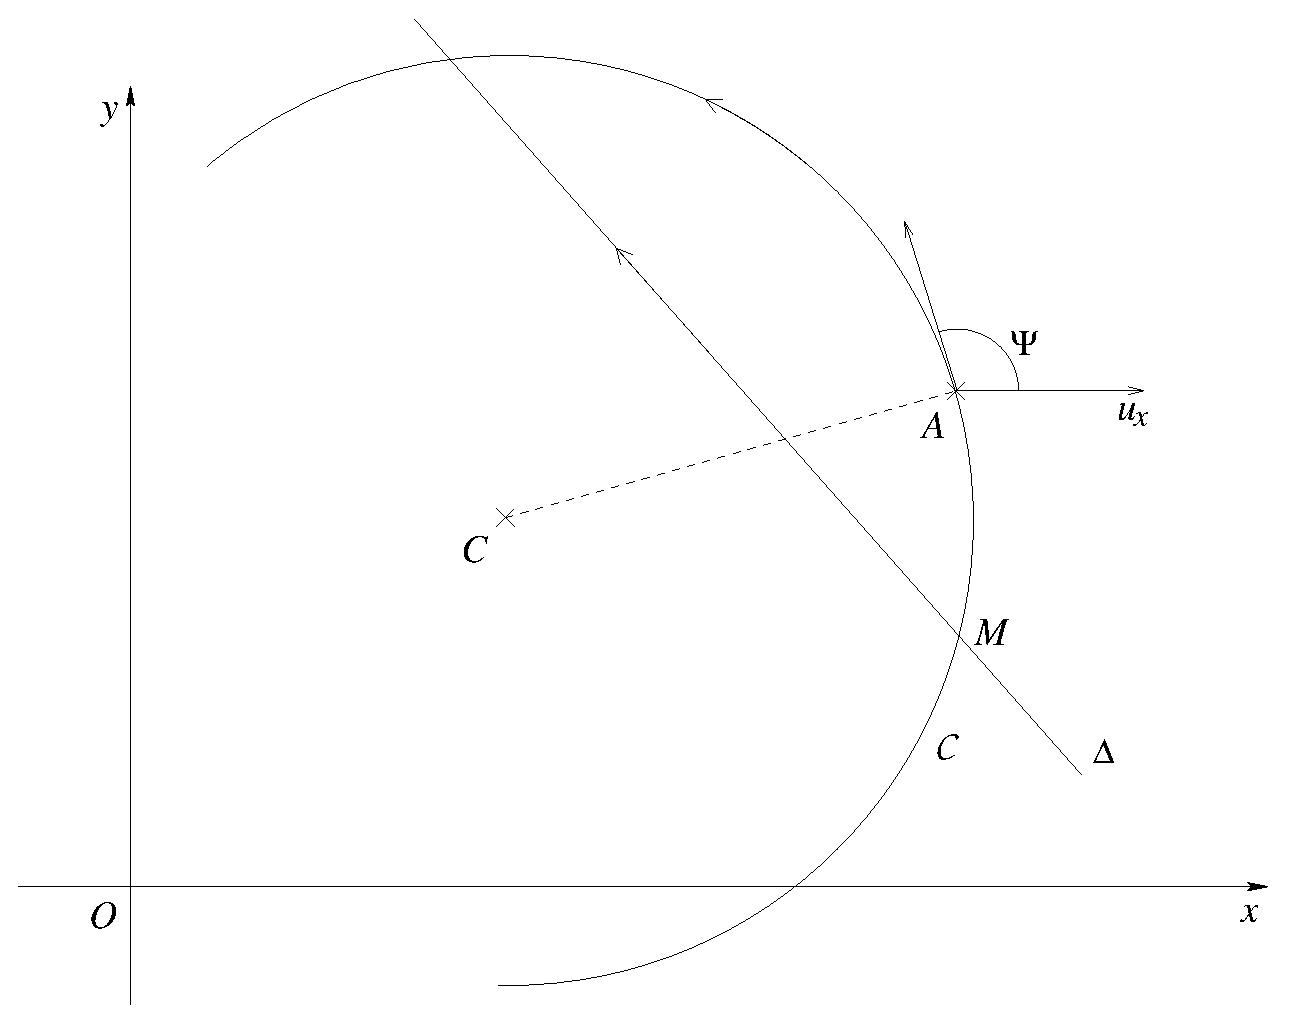
\epsfig{file=calcFig1.eps,width=11cm}

\mycaption{Projection of the cascade geometry in the 2-D plane (xOy)}
\label{calcFig1}
\end{center}

%{\small{\normalsize 
%The first part of the code that is run is the former subroutine {\tt update\_track\_param}. Its role is simply to move the orgin of the helix from its former position $A$ to its new position $M$ (actually, the point of the helix that overlaps with $M$ when projected to the $(xOy)$ plane).
%}\par}

%{\advance\baselineskip -5pt 
%The first part of the code that is run is the former subroutine {\tt update\_track\_param}. Its role is simply to move the orgin of the helix from its former position $A$ to its new position $M$ (actually, the point of the helix that overlaps with $M$ when projected to the $(xOy)$ plane).
%\par}

%{\setlength{\baselineskip}{0.2\baselineskip}
%The first part of the code that is run is the former subroutine {\tt update\_track\_param}. Its role is simply to move the orgin of the helix from its former position $A$ to its new position $M$ (actually, the point of the helix that overlaps with $M$ when projected to the $(xOy)$ plane).
%\par}

% Les 3 marchent, mais impossible de descendre en-dessous d'une certaine valeur !
% Au fait : ce que ca fait est que ca reduit (ou augmente) l'interligne.

The first part of the code that is run is the former subroutine {\tt update\_track\_param}. Its role is simply to move the orgin of the helix from its former position $A$ to its new position $M$ (actually, the point of the helix that overlaps with $M$ when projected to the $(xOy)$ plane).

%{\small{\normalsize 
% Pareil : ca descend pas en-dessous d'une certaine valeur, ici bien trop grande.
% Donc je me definis mon propre style de liste :-)
Here is a list of the various variables in this area of the code :
\begin{maliste}
\item {\tt axb} : $\overrightarrow{CA} \cdot \overrightarrow{w}$, where $\overrightarrow{w}$ is the vector such as $\|\overrightarrow{w}\| = \|\overrightarrow{CM}\|$ and $(\widehat{\overrightarrow{CM},\overrightarrow{w}}) = -\frac{\pi}{2}$
\item {\tt arg} : $\sin(\overrightarrow{CA},\overrightarrow{CM})$
\item {\tt ds} : curvilinear length on the {\em circle} between $A$ and $M$
\item {\tt dz} : $z_M - z_A$
\end{maliste}
And what follows is how to do the link between the code and the mathematical formulas~:\\
In the code, calling $xi$ and $yi$ the coordinates of the origin :\\
{\tt axb = (xi-xc)(yOut-yc) - (yi-yc)(xOut-xc)}
$$
\overrightarrow{CA} =
\left|\begin{array}{l}
x_{_A} - x_{_C} \\
y_{_A} - y_{_C} \\
\end{array}\right.
\qquad\qquad
\overrightarrow{CM} =
\left|\begin{array}{l}
x_{_M} - x_{_C} \\
y_{_M} - y_{_C} \\
\end{array}\right.
\qquad\qquad
\overrightarrow{w} =
\left|\begin{array}{l}
y_{_M} - y_{_C} \\
-(x_{_M} - x_{_C}) \\
\end{array}\right.
$$
So $\overrightarrow{CA} \cdot \overrightarrow{w} = (x_{_A}-x_{_C})(y_{_M}-y_{_C}) - (y_{_A}-y_{_C})(x_{_M}-x_{_C}) = \text{\tt axb}$.\\
%$\overrightarrow{w} \perp \overrightarrow{CM}$, so $\overrightarrow{w}$ drives the tangent to the circle in $M$.
Now, let's try to find what is this $\text{\tt axb} = \overrightarrow{CA} \cdot \overrightarrow{w}$~:\\
we know that $\|\overrightarrow{w}\| = \|\overrightarrow{CM}\|$, so~:
$$
\begin{array}{r@{\;=\;}l}
\overrightarrow{CA} \cdot \overrightarrow{w} & \|\overrightarrow{CA}\| \cdot \|\overrightarrow{w}\| \cos(\overrightarrow{CA},\overrightarrow{w}) \\
 & \|\overrightarrow{CA}\| \cdot \|\overrightarrow{CM}\| \cos((\overrightarrow{CA},\overrightarrow{CM}) + (\overrightarrow{CM},\overrightarrow{w})) \\
	& R^2 \cos((\overrightarrow{CA},\overrightarrow{CM}) - \frac{\pi}{2}) \\
	& R^2 \sin(\overrightarrow{CA},\overrightarrow{CM}) \\
\end{array}
$$
Therefore, since $\text{\tt rsq} = R^2$, we obtain $\text{\tt arg} = \text{\tt axb/rsq} = \sin(\overrightarrow{CA},\overrightarrow{CM})$.\\
{\tt ds} is then defined as the angle ($\arcsin(\text{\tt arg})$) multiplied by $R$, i.e. it is the curvilinear length on the circle from $A$ to $M$.\\
And then, from the definition of the dip angle\footnote{For a detailed note about the helices' parameters, see the appendix A of the Star Class Library documentation.\label{SCL}}, 
%\footnotemark[1]
we obtain that {\tt dz = ds.tan(dipAngle)} is $z_M - z_A$ (considering this time $A$ and $M$ as the points on the helix instead of on the circle).
%}\par}
%\footnotetext[1]{For a detailed note about the helices' parameters, see the appendix A of the Star Class Library documentation.}

At the end of the former subroutine {\tt update\_track\_param}, a helix called {\tt bachGeom2} is booked with the same parameters than the original bachelor helix taken from the track container, {\tt bachGeom}, except for the origin that has been moved from $A$ to $M$, and the angle $\Psi$ that obviously changes when the origin moves (see {\sc Fig.} \ref{calcFig1}).

The next piece of code is the former subroutine {\tt track\_mom}, which just books the momentum of the bachelor taken in $M$ in the variable {\tt xOrig} (which contained the 3-D position of $M$ a couple of code-lines before~: since both usages don't overlap, the same StThreeVector can be used for both of them).

The next part of the code is the most difficult one to understand. It wasn't a subroutine in the Fortran code~: that was part of the {\tt exiam} function.
Here is a list of the various variables in this area of the code~:
\begin{maliste}
\item {\tt pBach} : normalised momentum of the bachelor in $M$ (so it's rather the (normalised) direction of the tangent to the helix in $M$)
\item {\tt dv0dotdb} : $\cos (\overrightarrow{\text{\tt dpV0}},\overrightarrow{\text{\tt pBach}})$
\item {\tt diffc} : $\overrightarrow{MV}$, calling $V$ the point where the V0 decays
\item {\tt denom} : $\cos^2 (\overrightarrow{\text{\tt dpV0}},\overrightarrow{\text{\tt pBach}}) - 1$
\item {\tt s2} : ehm... well... see the explanations below !
\item {\tt valid} : relative error due to the linearisation
\end{maliste}
So let's call $V$ the position of the V0 vertex, i.e. the point where the V0 decays. As described p. \pageref{linearisation}, we now linearise the helix, i.e. we assume that the helix can be merged with its tangent in $M$ (in 3-D). So an approximation of the point where the distance between the helix and the V0 line is the smallest is the point where the distance between the tangent to the helix and the V0 line is the smallest.

Let $\mathcal D$ be the tangent to the helix in $M$, $\Delta$ being the V0 line, and let $H_1$ (resp. $H_2$) be the point on $\Delta$ (resp. on $\mathcal D$) where the distance to $\mathcal D$ (resp. to $\Delta$) is the smallest. A 3-D illustration with those points can be seen on {\sc Fig.} \ref{calcFig3}.

Calling $\overrightarrow{u}$ the vector that drives $\Delta$ (i.e. $\overrightarrow{u} = \overrightarrow{\text{\tt dpV0}}$) and $\overrightarrow{v}$ the vector that drives $\mathcal D$ (i.e. $\overrightarrow{v} = \overrightarrow{\text{\tt pBach}}$), we can write $H_1$ and $H_2$ as~:
$$
H_1 = V + k_1 \overrightarrow{u}
\qquad\qquad
H_2 = M + k_2 \overrightarrow{v}
$$
With the definition of $H_1$ and $H_2$ above, we can write that we search~:
\begin{equation}\label{k1k2}(H_1 \in \Delta , H_2 \in {\mathcal D}) \quad / \quad \overrightarrow{H_1 H_2} \perp \Delta \quad \text{and} \quad \overrightarrow{H_1 H_2} \perp {\mathcal D}
\end{equation}
\begin{equation}\label{Systeme}
\Leftrightarrow \quad (H_1 \in \Delta , H_2 \in {\mathcal D}) \quad / \quad \overrightarrow{H_1 H_2} \cdot \overrightarrow{u} = \overrightarrow{H_1 H_2} \cdot \overrightarrow{v} = 0
\end{equation}
Given that
$$\begin{array}{r@{\;=\;}l}
\overrightarrow{H_1 H_2} & M + k_2 \overrightarrow{v} - V - k_1 \overrightarrow{u} \\
& \overrightarrow{VM} + k_2 \overrightarrow{v} - k_1 \overrightarrow{u} \\
& -\overrightarrow{\text{\tt diffc}} + k_2 \overrightarrow{v} - k_1 \overrightarrow{u} \\
\end{array}$$
we can re-write the system \eqref{Systeme} as
$$\left\{\begin{array}{r@{\;=\;}l@{\;=\;}l}
\overrightarrow{H_1 H_2} \cdot \overrightarrow{u} & -\overrightarrow{\text{\tt diffc}} \cdot \overrightarrow{u} + k_2 \overrightarrow{v} \cdot \overrightarrow{u} - k_1 \overrightarrow{u} \cdot \overrightarrow{u} & 0 \\
\overrightarrow{H_1 H_2} \cdot \overrightarrow{v} & -\overrightarrow{\text{\tt diffc}} \cdot \overrightarrow{v} + k_2 \overrightarrow{v} \cdot \overrightarrow{v} - k_1 \overrightarrow{u} \cdot \overrightarrow{v} & 0 \\
\end{array}\right.$$
which can also be written as
$$\left\{\begin{array}{r@{\;=\;}l}
-\overrightarrow{\text{\tt diffc}} \cdot \overrightarrow{u} + k_2 \cos(\overrightarrow{v},\overrightarrow{u}) - k_1 & 0 \\
-\overrightarrow{\text{\tt diffc}} \cdot \overrightarrow{v} + k_2 - k_1 \cos(\overrightarrow{u},\overrightarrow{v}) & 0 \\
\end{array}\right.$$
because $\|\overrightarrow{u}\| = \|\overrightarrow{v}\| = 1$.\\

\begin{center}

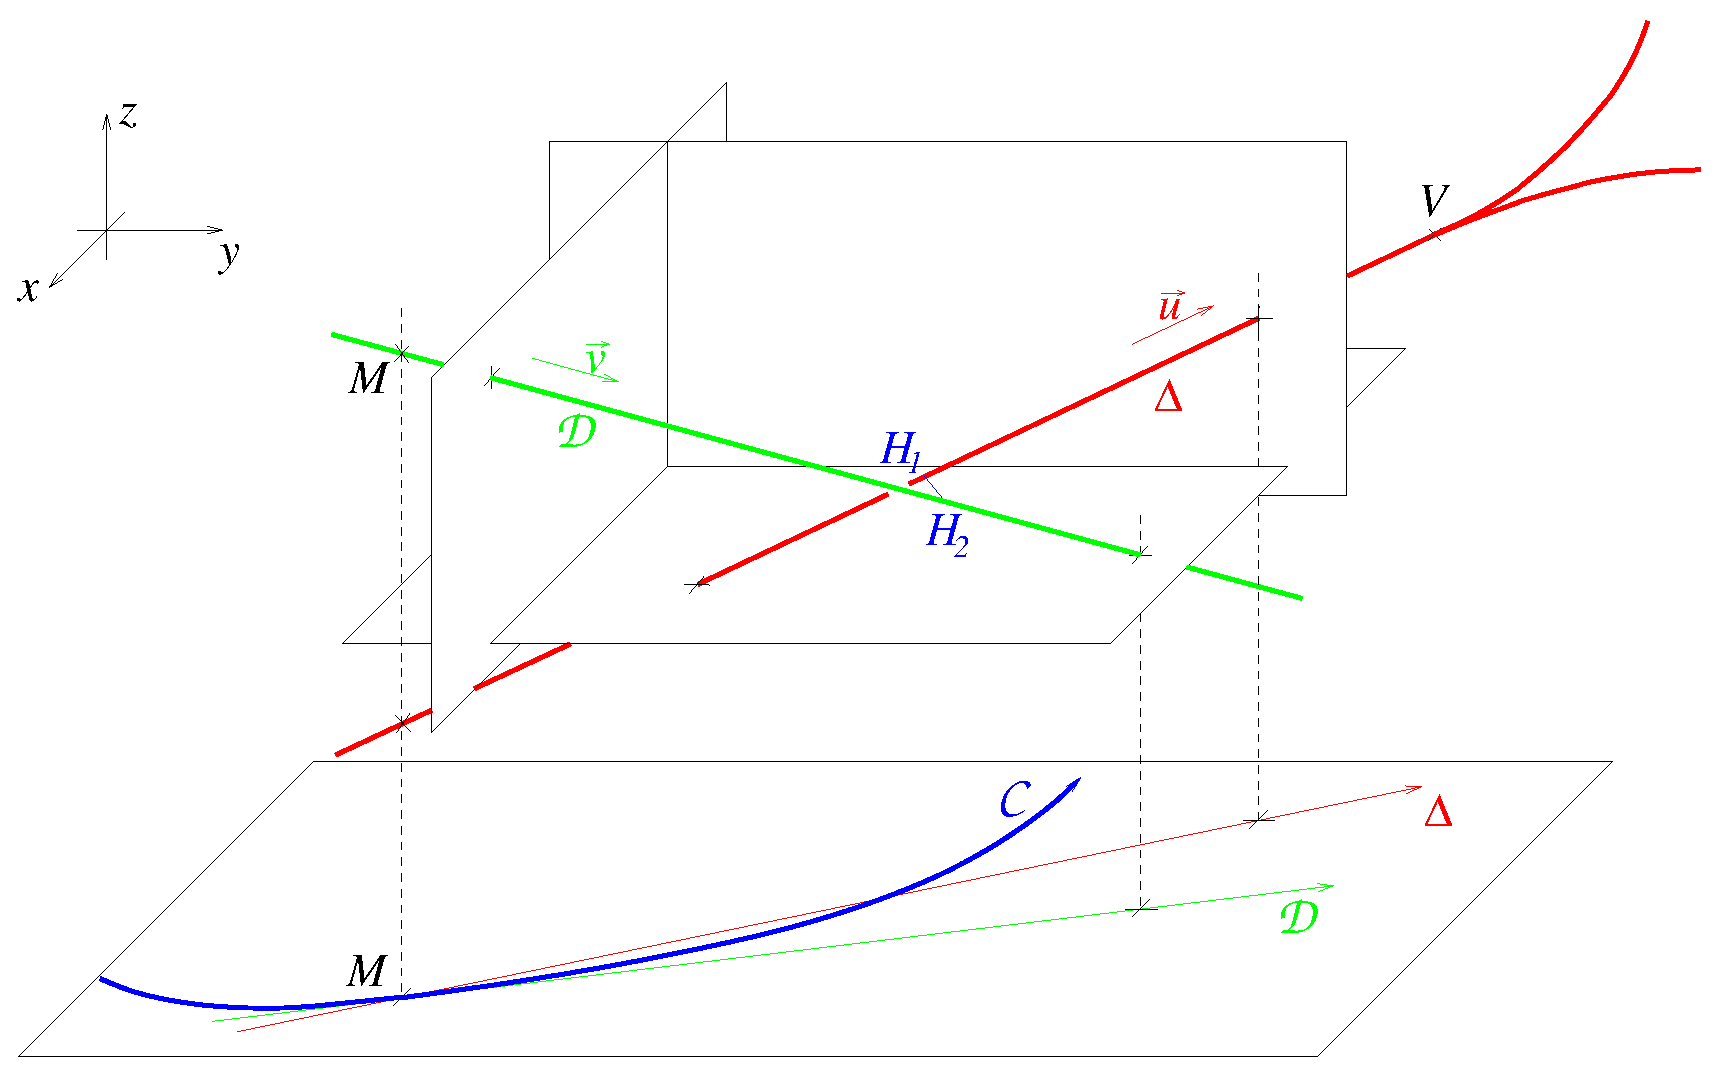
\epsfig{file=calcFig3.eps,width=15cm}

\mycaptionBis{3-D illustration of lines and points' names introduced in the text}{3-D illustration of lines and points' names introduced in the text. The V0 is in red, the projection of the helix in the bending plane is in blue, and the tangent to this helix is in green}
\label{calcFig3}
\end{center}

{\parindent=0pt Solving this system, we obtain :
$$\left\{\begin{array}{r@{\;=\;}l}
 k_1 & \frac{\strut -\overrightarrow{\text{\tt diffc}} \cdot (\overrightarrow{v}\cos(\overrightarrow{u},\overrightarrow{v}) - \overrightarrow{u})}{\strut \cos^2 (\overrightarrow{u},\overrightarrow{v}) - 1} \\
k_2	& \frac{\strut \overrightarrow{\text{\tt diffc}} \cdot (\overrightarrow{u}\cos(\overrightarrow{u},\overrightarrow{v}) - \overrightarrow{v})}{\strut \cos^2 (\overrightarrow{u},\overrightarrow{v}) - 1} \\
\end{array}\right.$$
In the code, {\tt s2} is calculated as :\\
{\tt s2 = (dpV0.X dv0dotdb - pBach.X) diffc.X + (dpV0.Y dv0dotdb - pBach.Y) diffc.Y + \\
\hspace*{20pt} + (dpV0.Z dv0dotdb - pBach.Z) diffc.Z;}\\ %"hspace*" au lieu "hspace" pour le forcer en debut de ligne.
{\tt s2 = s2/denom;}\\
which can be written as\footnote{Given that $\text{\tt dv0dotdb} = \overrightarrow{\text{\tt dpV0}} \cdot \overrightarrow{\text{\tt pBach}} = \cos (\overrightarrow{\text{\tt dpV0}},\overrightarrow{\text{\tt pBach}})$. Thus $\text{\tt denom} = \cos^2 (\overrightarrow{\text{\tt dpV0}},\overrightarrow{\text{\tt pBach}}) -1 = \cos^2 (\overrightarrow{u},\overrightarrow{v}) - 1$.} :
$$\begin{array}{r@{\;=\;}l}
\text{\tt s2} & \frac{\strut (\overrightarrow{\text{\tt dpV0}} \cos(\overrightarrow{u},\overrightarrow{v}) - \overrightarrow{\text{\tt pBach}}) \cdot \overrightarrow{\text{\tt diffc}}}{\strut \cos^2 (\overrightarrow{u},\overrightarrow{v}) - 1} \\
 & \frac{\strut \overrightarrow{\text{\tt diffc}} \cdot (\overrightarrow{u} \cos(\overrightarrow{u},\overrightarrow{v}) - \overrightarrow{v})}{\strut \cos^2 (\overrightarrow{u},\overrightarrow{v}) - 1} \\
	& k_2 \\
\end{array}$$
So {\tt s2} is the 3-D algebraic distance $\overline{MH_2}$ between $M$ and $H_2$, the point of $\mathcal D$ that is closest to $\Delta$.}

Then, {\tt valid} is calculated as $\left|\text{\tt s2} \sqrt{\text{\tt pBach.X}^2 + \text{\tt pBach.Y}^2}\right|$, i.e. it's the distance in the $(xOy)$ plane between $M$ and $H_2$, as illustrated by figure \ref{calcFig2}. The value {\tt valid} itself is not very helpful to determine if the linearisation is a good approximation or not. The value that has to be looked at is actually the distance between $H_2$ and the circle in the 2-D plane, which is called $d$ in figure \ref{calcFig2}.

But $d$ actually depends explicitely on {\tt valid}, which means that an initial requirement on $d$ can be transformed into a requirement on {\tt valid}. This allows not to calculate $d$ and saves some calculation time -- at least it's the only reason I've found that would explain why the authors of the code have chosen to test {\tt valid} rather than $d$ ! The relation between $d$ and {\tt valid} is~:
$$d = \sqrt{R^2 + \text{\tt valid}^2} - R$$
\begin{equation}\label{dVsValid}
\Leftrightarrow \quad \frac{d}{R} = \sqrt{1+\left(\frac{\text{\tt valid}}{R}\right)^2\:} - 1
\end{equation}

There are 2 conditions on $\frac{\text{\tt valid}}{R}$. Let's call these two values $valid_1$ and $valid_2$, with $valid_1 < valid_2$. The original algorithm (it may be changed in the mid-future) throws away any Xi candidate for which $\text{\tt valid} > valid_2$, and keeps all the other ones. But if $\text{\tt valid} \in [valid_1 ; valid_2]$, then another part of the algorithm, which is described in the next paragraph, is run. It consists in improving the quality of the linearisation by linearising the helix at another point. This improvement is tried at most 3 times. Basically, this means that a linearisation that gives $\text{\tt valid} > valid_2$ means that it's hopelessly bad~; when $\text{\tt valid} < valid_1$ it means that the linearisation is good enough and doesn't need to be improved~; and when $\text{\tt valid} \in [valid_1 ; valid_2]$, the linearisation is improved but it actually doesn't matter if the criterium $\text{\tt valid} < valid_1$ is not reached~: the candidate is kept anyway. According to the tests, only a very few proportion of the candidates need 3 passes in the loop\footnote{Result obtained over 1 {\tt Au}-{\tt Au} $200~GeV$ central event~: over 73 269 bachelors, neglecting those which have only 1 intersection point, 45 500 have 2 intersection points, i.e. 62 \% of them (and therefore 38 \% have no intersection points). Among the 118 194 dca calculations of those 62 \%, 77.0 \% of them don't need a better linearisation, 21.7 \% need to go once in the loop, 0.8 \% need to go twice in the loop, and 0.5 \% go 3 times in the loop (this latter percentage, unike the former ones, is the number of candidates that need only 3 passes added to the number of candidates that would need more).}, so requiring more than 3 passes is indeed not necessary.

\begin{center}
\begin{tabular}{lc}
% Il sait pas wrapper !! Pour le faire, il faut charger le package multirow, mais je peux pas utiliser de package pour cette doc...
% Et en plus je suis oblige de mettre dans un tableau, ligne par ligne, sinon il met le tableau de la 2e partie aligne avec la 3e ligne de texte... Je pourrais me demerder avec une box, mais c'est chiant et pas propre non plus...
\begin{tabular}{l}
This table shows the numerical values of $valid_1$ and $valid_2$ \\
used in the code (first line) and their equivalent for the more \\
interesting variable $\frac{d}{R}$, calculated with \eqref{dVsValid}.\\
\end{tabular}
&
\begin{tabular}{r@{~$<$~}c@{~$<$~}l}
$0.001~R$ & {\tt valid} & $0.02~R$ \\
$5.10^{-7}~R$ & $d$ & $2.10^{-4}~R$ \\
0.0005 \% & $\frac{d}{R}$ & 0.02 \% \\
\end{tabular}
\\
\end{tabular}
\end{center}

So when $\text{\tt valid} \in [valid_1 ; valid_2]$, here is the piece of code that is run~:
\begin{maliste}
\item Former subroutine {\tt ev0\_project\_track} : calculates the coordinates (in the $(xOy)$ plane) of the point $M'$ defined as the intersection of the circle $\mathcal C$ and the line $(CH_2)$ (see {\sc Fig.} \ref{calcFig2})
\item Former subroutine {\tt update\_track\_param} : moves the origin of the helix from $M$ to $M'$ (as previously done from $A$ to $M$)
\item Former subroutine {\tt track\_mom} : calculates the momentum of the bachelor in $M'$ (as previously done in $M$)
\item Block that calculates {\tt s2} and {\tt valid} : calculates a new {\tt s2} and {\tt valid}, whose value will be checked to see if one more pass in this loop is necessary
\end{maliste}

\begin{center}

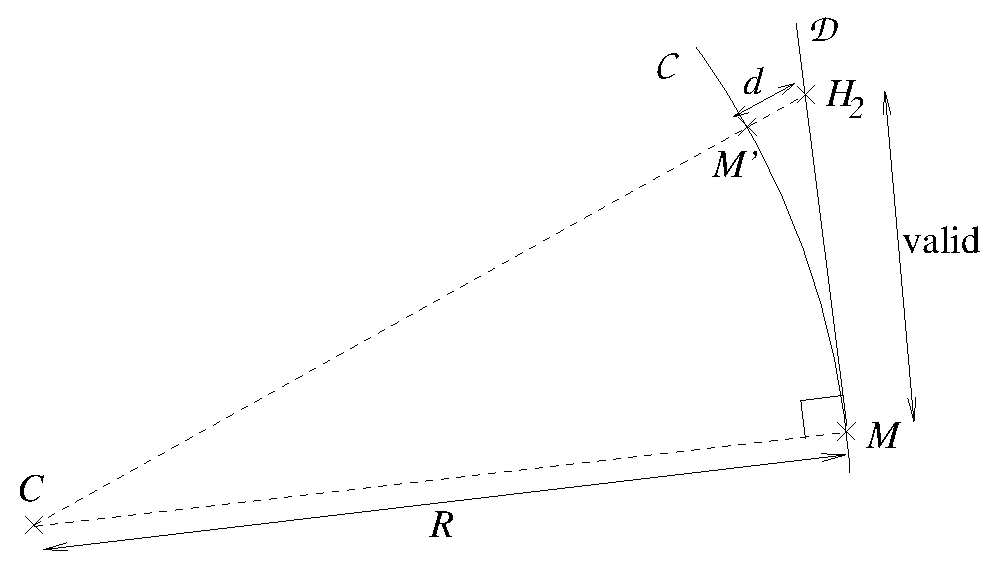
\epsfig{file=calcFig2.eps,width=11cm}

\mycaption{2-D plane evaluation of the quality of the approximation made by linearising the helix}
\label{calcFig2}
\end{center}

The 3 last blocks are exactly the same as those already described above, so I'll only describe the former subroutine {\tt ev0\_project\_track}~: the list below is made of the variables that are used in this area of the code~:
\begin{maliste}
\item {\tt batv} : 3-D coordinates of $H_2$
\item {\tt dtmp} : $x_{_C} - x_{_{H_2}}$
\item {\tt atmp} : $y_{_C} - y_{_{H_2}}$
\item {\tt ctmp} : slope of the line $(CH_2)$
\item {\tt yy} : $y_{_{M'}} - y_{_C}$
\item {\tt zz} : $x_{_{M'}} - x_{_C}$
\item {\tt xAns} : temporary variable, actually equal to xOut
\item {\tt yAns} : temporary variable, actually equal to yOut
\item {\tt xOut} : $x_{_{M'}}$ (contained $x_{_M}$ before)
\item {\tt yOut} : $y_{_{M'}}$ (contained $y_{_M}$ before)
\end{maliste}
The calculation of $(x_{_{M'}},y_{_{M'}})$ is simple : since $\text{\tt ctmp} = \frac{x_{_C} - x_{_{H_2}}}{y_{_C} - y_{_{H_2}}}$ is the inverse of the slope of $(CH_2)$ the equation of $(CH_2)$ is~:
$$(CH_2) : y = \frac{1}{\text{\tt ctmp}}(x - x_{_C}) + y_{_C}$$
and therefore, setting $x' = x_{_{M'}} - x_{_C}$ and $y' = y_{_{M'}} - y_{_C}$, $M'$ is such as~:
$$\left\{\begin{array}{l}
y' = \left(\frac{1}{\text{\tt ctmp}}\right)x' \\
{x'\strut }^2 + {y'\strut }^2 = R^2 \\
% strut pour separer un peu mieux les 2 lignes du systeme, et accolades obligatoires pour x'^2 car il accepte pas un ^ juste apres un ^ (il considere que c'est 2 superscripts).
\end{array}\right.$$
Solving this system gives :
$$\left\{\begin{array}{r@{\;=\;}l}
y' & \pm \frac{R}{\sqrt{1+\text{\tt ctmp}^2}} \\
x' & \text{\tt ctmp}\cdot y' \\
\end{array}\right.$$
$x'$ and $y'$ are respectively {\tt zz} and {\tt yy} in the code, and the ``signus dilemma" is solved by the if-loop on the sign of {\tt atmp}.

And here is eventually the list of the variables used at the end of the code~:
\begin{maliste}
\item {\tt v0atv} : 3-D coordinates of $H_1$
\item {\tt s1} : see the explanations below and page \pageref{k1k2}
\item {\tt xOrig} : momentum of the bachelor at $H_2$ (be careful~: at other places of the code, {\tt xOrig} actually stores the origin of the bachelor's helix)
\item {\tt dca} : $d_{H_1 H_2}^2 = \left\|\overrightarrow{\text{\tt v0atv} - \text{\tt batv}}\right\|^2$~: it's the (squared) approximated distance of closest approach between the Lambda and the bachelor. Keeping the squared value and taking the root only at the moment of storing the value avoids time-consuming square-root calculations before all the final cuts
\item {\tt xpp} : position of the Xi decay point : it's the middle of $[H_1 H_2]$, i.e. $\frac{\text{\tt v0atv} - \text{\tt batv}}{2}$
\item {\tt rv} : the Xi decay length ($\left\|\overrightarrow{\text{\tt xpp} - \text{\tt xPvx}}\right\|$), used only in the former versions of the code (and in Fortran). Now, the cut on the decay length is done ``on the fly"
\item {\tt pXi} : momentum of the reconstructed Xi : $\overrightarrow{p_{_{Xi}}} = \overrightarrow{p_{_{V0}}} + \overrightarrow{p_{_{Bach,H_2}}}$
\item {\tt check} : used only in Fortran and in the former versions of the C++ code~: contains first $\overrightarrow{H_1 V} \cdot \overrightarrow{p_{_{V0}}}$ (({\tt xV0} - {\tt v0atv}) . $\overrightarrow{\text{\tt pV0}}$), and then $\overrightarrow{PvxXivtx} \cdot \overrightarrow{p_{_{Xi}}}$ (({\tt xpp} - {\tt xPvx}) . $\overrightarrow{\text{\tt pXi}}$) to check that the V0 points away from the Xi vertex and the Xi points away from the primary vertex
\item {\tt pper} : $p_\perp$ Armanteros of the Xi
\item {\tt globHelix} : temporary {\tt StHelix} booked with temporary variables (their name end in {\tt \_tmp}), used to calculate {\tt bxi} with StEvent functions
\item {\tt bxi} : distance of closest approach between the Xi and the primary vertex
\end{maliste}

At the end of the while-loop, the candidates for which $\text{\tt valid} > valid_2$ are simply thrown away, and all the other ones are kept, even if $\text{\tt valid} > valid_1$. The value of {\tt s2} calculated during the last loop is kept, and {\tt s1} (which is the $k_1$ of equation \eqref{k1k2} (p. \pageref{k1k2}) and of the following ones) is calculated as
$$\text{\tt s1} = \frac{-\overrightarrow{\text{\tt diffc}} \cdot (\overrightarrow{\text{\tt pBach}} \times \text{\tt dv0dotdb} - \overrightarrow{\text{\tt dpV0}})}{\text{\tt dv0dotdb}^2 - 1} = \frac{-\overrightarrow{\text{\tt diffc}} \cdot (\overrightarrow{v}\cos(\overrightarrow{u},\overrightarrow{v}) - \overrightarrow{u})}{\cos^2(\overrightarrow{u},\overrightarrow{v}) - 1} = k_1$$
Then, the 3-D coordinates of $H_1$ are calculated and stored in {\tt v0atv}, just like the coordinates of $H_2$ are stored in {\tt batv}. Once this is done, we check that $\overrightarrow{H_1 V}$ goes roughly in the same direction as $\overrightarrow{p_{_{V0}}}$, i.e. that the V0 points away from the Xi vertex newly found. This was formerly done via the variable {\tt check}, that is exactly $\overrightarrow{H_1 V} \cdot \overrightarrow{p_{_{V0}}}$, but is now done ``on the fly".

If {\tt check} is positive, it means that the V0 points to the opposite direction than where the Xi vertex is, and the rest of the algorithm -- run only in that case -- can be roughly summed up as something that looks like this for the latest versions of the code~:

$$
\begin{array}{|ll|}
\hline
\hspace{4pt}~ &

\hspace{-10pt}
\begin{tabular}{l}
Calculate some cut variables \\
if (cuts are not OK) {\tt continue} \\
{\tt pXi} = {\tt pV0} + {\tt xOrig} \\
if (Xi doesn't point away from primary vertex) {\tt continue} \\
Calculate $p_\perp$ Armanteros, cut on it \\
Calculate signed dcaXiToPrimaryVertex, cut on it \\
Store the candidate \\
\end{tabular} \\

\hline
\end{array}
$$

{\parindent0pt and like that for the former versions of the code as well as for the Fortran program~:}

$$
\begin{array}{|ll|}
\hline
\hspace{4pt}~ &

\hspace{-10pt}
\begin{tabular}{l}
{\tt dca} = $\left\|\overrightarrow{\text{\tt v0atv} - \text{\tt batv}}\right\|$ \hspace{55pt} {\tt // }{\tt dca} = $H_1 H_2$ \\
{\tt xpp} = $\frac{\text{\tt v0atv} - \text{\tt batv}}{2}$ \hspace{85pt} {\tt // }{\tt xpp} = 3-D coordinates of the middle of $[H_1 H_2]$ \\
{\tt rv} = $\left\|\overrightarrow{\text{\tt xpp} - \text{\tt xPvx}}\right\|$ \hspace{72pt} {\tt // }{\tt rv} = Xi decay length \\
if (cuts are OK) \\
\end{tabular} \\

\hspace{4pt}~ &
\left \lfloor
\begin{array}{l}

\hspace{-10pt}
\begin{tabular}{l}
{\tt pXi} = {\tt pV0} + {\tt xOrig} \hspace{58pt} {\tt // }$\overrightarrow{p_{_{Xi}}} = \overrightarrow{p_{_{V0}}} + \overrightarrow{p_{_{Bach,H_2}}}$\\
{\tt check} = ({\tt xpp} - {\tt xPvx}) . $\overrightarrow{\text{\tt pXi}}$ \hspace{20pt} {\tt // }Check that $\overrightarrow{PvxXivtx} \cdot \overrightarrow{p_{_{Xi}}} \geq 0$, i.e. that the \\
if ({\tt check} $\geq$ 0) \hspace{84pt} {\tt // } \hspace{20pt} reconstructed Xi points away from the Pvx \\
\end{tabular} \\

\left \lfloor
\begin{tabular}{l}
{\tt iflag}=0 if the dcaXiToPrimaryVertex (cut) is OK \\
\end{tabular}
\right. \\

\hspace{-10pt}
\begin{tabular}{l}
if ({\tt iflag}=0) \\
\end{tabular} \\

\left \lfloor
\begin{tabular}{l}
Calculates the kinematic variables \\
Calculate unsigned dcaXiToPrimaryVertex, cut on it \\
Store the candidate \\
\end{tabular}
\right. \\

\vspace{-12pt}
\end{array}
\right. \\
\hline
\end{array}
$$










\subsubsection{Detailed algorithm and cuts}

The detailed algorithm is actually explained in the section \ref{paragrDca} concerning the calculation of the dca, p. \pageref{paragrDca}. Yet, in the latter paragraph, no overview of the algorithm is given and the cuts are not listed. This is the purpose of this short paragraph, and is summed up in {\sc Fig}. \ref{XiAlgoMieux}.

\begin{center}

$
\begin{array}{|ll|}
\hline
\hspace{4pt}~ &
\hspace{-10pt} \begin{tabular}{l} Prepare things via the V0Finder \\ {\bf Loop} over V0 vertices \\ \end{tabular} \\
\hspace{4pt}~ &
\left \lfloor
\begin{array}{l}

\hspace{-10pt}
\begin{tabular}{l}
Get event- and V0-wise information \\
{\footnotesize\bf CUT \hspace{-30pt} CUT} on the (false) V0 decay length (distance to primary) \\
Prepare rotating variables \\
Calculates Lambda invariant mass ; decide if $\Lambda$ or $\overline{\Lambda}$ \\
{\footnotesize\bf CUT \hspace{-30pt} CUT} on $\Lambda$ invariant mass \\
Prepare like-sign variable (change {\tt charge}) \\
{\bf Loop} over global tracks \\
\end{tabular} \\

\left \lfloor
\begin{tabular}{l}
{\bf If} {\em track has wrong charge} : next \\
Select {\sc tpt} vs {\sc ittf} tracks \\
{\bf If} {\em track already used in the V0} : next \\
Determine Xi's detector {\sc id} \\
Find {\sc dca} between V0's straight line and track's helix \\
\hfill (Implies {\footnotesize\bf CUT \hspace{-30pt} CUT} on number of intersection points \\
\hfill and {\footnotesize\bf CUT \hspace{-30pt} CUT} on validity of linearisation) \\
{\footnotesize\bf CUT \hspace{-30pt} CUT} if V0 doesn't point away from Xi vertex \\
{\footnotesize\bf CUT \hspace{-30pt} CUT} on dca between V0 and bachelor \\
{\footnotesize\bf CUT \hspace{-30pt} CUT} on Xi decay length \\
{\footnotesize\bf CUT \hspace{-30pt} CUT} if Xi doesn't point away from primary vertex \\
{\footnotesize\bf CUT \hspace{-30pt} CUT} on $p_\perp$ Armanteros \\
{\footnotesize\bf CUT \hspace{-30pt} CUT} on dcaXiToPrimaryVertex \\
Fill an {\tt StXiVertex} \\
Store it \\
\end{tabular}
\right. \\
\vspace{-10pt}
\end{array}
\right. \\
\hline
\end{array}
$

\mycaption{Cuts and algorithm of the XiFinder}
\label{XiAlgoMieux}

\end{center}

A short comment : variable {\tt charge} is the sign of the bachelor, so when no like-sign is required, {\tt charge} is also the sign of the Xi~: {\tt charge} $ = -1$ for $\Xi$ and $\Omega$, $+1$ for $\overline{\Xi}$ and $\overline{\Omega}$.

As for the V0Finder, a cut has been introduced compared to the Fortran version, on Feb 5th 2004~: the cut on the $p_\perp$ Armanteros. It removes 19 \% of the candidates (all background), so this cut used with the cut on the number of hits of the bachelor's track\footnote{Implemented in the V0Finder, although it concerns only the XiFinder. See \S\ \ref{cutNTH} p. \pageref{cutNTH} for more information.} remove 34 \% of the background.
\label{cutPtArm}








\vspace{1cm}

\section{Magnetic field}

The magnetic field is calculated from the first track stored in the track table, in {\tt StV0FinderMaker::\-Pre\-pare()}. Its sign is simply taken from the charge and the helicity~:
$$\text{sgn}(B) = - \text{sgn}(charge) \times \text{sgn}(helicity)$$
while the absolute value is calculated from the momentum of the track~: an arbitrary value is given to the magnetic field ($1.10^{-10}$ in the current version of the code)~; then, assuming this value for $\overrightarrow{B}$, the momentum of the track is calculated from its geometrical characteristics (curvature of the helix), by using a function of StEvent. This value is compared to the actual momentum of this track, and the ratio between both momenta simply gives the factor to apply to the arbitrary value given to $\overrightarrow{B}$ to get the real magnetic field~:\\
$B = 1.10^{-10}$ \\
$\overrightarrow{p_1}$ = actual momentum of the particle \\
$\overrightarrow{p_2}$ = momentum associated to the track assuming $B$ \\
Actual $B$ = $B \times \frac{p_1}{p_2}$

The magnetic field algebraic value is stored in the member-variable {\tt Bfield}. The value of {\tt tesla} is $1.10^{-13}$, that of {\tt kilogauss} is $1.10^{-14}$.

If one wants to get the magnetic field value from gufld, it's still possible~: the lines mentionned above need of course to be commented out, and 3 pieces of codes just need to be uncommented~:
\begin{maliste}
\item 3 lines ({\tt include}, {\tt extern}, {\tt define}) at the very beginning of {\tt V0Finder.cxx}
\item function {\tt InitRun} in {\tt V0Finder.cxx} and {\tt V0Finder.h}
\end{maliste}
and Geant has to be instantiated in the macro that calls the V0/XiFinders (if you use the BFC~: no worry, it works right away).








\vspace{1cm}

\section{Detectors}

Each track has a {\em detector ID}, an integer that tells in which detectors this track has been seen. The detector {\sc id} of each track is stored in the table {\tt detId}\footnote{Not to be mixed up with table {\tt trkID}, in which the {\em keys} of the tracks are stored.} (filled in {\tt StV0FinderMaker::Prepare()}).

The table below sums up the various states of this flag, for tracks that have a hit in the {\sc tpc} only, in the {\sc svt} only, or in both detectors.
\begin{center}
\begin{tabular}{|c|c|c|}
\hline
{\tt detId} & Hit(s) in TPC & Hit(s) in SVT \\
\hline
1 & X &   \\
2 &   & X \\
3 & X & X \\
\hline
\end{tabular}
\end{center}
Case 2 should not happen this days since the SVT doesn't create tracks up to now, but this may become possible, so the possibility for SVT-only tracks is kept. In this paragraph, ``SVT" actually means ``SVT and/or SSD".

The detector {\sc id} of the V0 and of the Xi are respectively stored in the member-variables {\tt det\_id\_v0} and {\tt det\_id\_xi}. Both of them are equal to the higher of their 2 daughters' detector {\sc id}. This means that for example a Xi will have a detector {\sc id} of 3 whatever the number of its 3 daughters that have at least 1 hit in the SVT (provided that at least one of them has a hit in the SVT).



\subsection{Cut values}

The cut values depend on various things :
\begin{maliste}
\item The collision system : of course, way looser cuts are needed for e.g. {\tt p-p} than for {\tt Au-Au}
\item The detector {\sc id} : e.g. the position of a Xi vertex is better determined when the SVT is used
\item For the V0s : the fact that they are primary or secondary~; the cut on the false decay length (distance between the primary vertex and the V0 decay point) is tighter for primary V0's, because we want them to come from the primary vertex.
\end{maliste}

The numerical values of the cuts can be found in several files that are stored in directory {\tt StarDb/global/vertices/}. There is one file per collision system and energy. Files for the V0 cuts have a name that begins by {\em ev0par2}, and those for the Xi cuts have a name that begins by {\em exipar}.

A V0 file has 2 times 3 sets of cuts. The first 3 sets are cuts used for all the V0s (primary and secondary), and the last 3 sets are tighter cuts used only for the primary V0s. The 3 sets are for (in this order)~:
\begin{maliste}
\item Tracks that have hits only in the TPC
\item Tracks that have hits only in the SVT
\item Tracks that have hits in both the TPC and the SVT
\end{maliste}
A Xi file has only 3 sets of cuts, because all the Xis are primary. The 3 sets are also TPC-only cuts, SVT-only cuts and TPC+SVT cuts.

Here is the composition of each set of cuts, for the V0's ({\em dca} stands for {\em distance of closest approach})~:
\begin{maliste}
\item {\tt dca} : maximum value of the dca between the two daughter tracks ;
\item {\tt dcav0} : maximum value of the dca between the V0 and the primary vertex (impact parameter)~;
\item {\tt dlen} : minimum value of the V0 false decay length (distance from the primary vertex to the decay point)~;
\item {\tt alpha\_max} : maximum absolute value of $\alpha_{Arm}$ ;
\item {\tt ptarm\_max} : maximum value of $p_{\perp Arm}$ ;
\item {\tt dcapnmin} : minimum value of the dca between the daughter tracks and the primary vertex (impact parameter)~;
\item {\tt iflag} : not used ;
\item {\tt n\_point} : minimum number of points on the track.
\end{maliste}
And here is that for the Xi's :
\begin{maliste}
\item {\tt use\_pid} : not used ;
\item {\tt dca\_max} : maximum value of the dca between the two daughters ;
\item {\tt bxi\_max} : maximum value of the dca between the Xi and the primary vertex (impact parameter)~;
\item {\tt rv\_xi} : minimum value of the Xi decay length ;
\item {\tt rv\_v0} : minimum value of the V0 false decay length (distance from the primary vertex to the decay point)~;
\item {\tt dmass} : cut the V0 invariant mass : keep a window of $\pm$ dmass around the mass of the Lambda~;
\item {\tt bpn\_v0} : minimum value of the dca between the pion daughter of the V0 and the primary vertex (impact parameter)~;
\item {\tt pchisq} : not used.
\end{maliste}

In the code, the Xi cut values are stored in the member-variable {\tt parsXi}, and the V0 cut values are stored in {\tt pars} and {\tt pars2}, respectively for the primary V0's and for all (primary and secondary) the V0's, both being member-variables.



\subsection{Using the SVT hits}

To be written.








\vspace{1cm}

\section{Rotating and like-sign}
\label{LikesignRotatingUsage}

These options have been implemented for analysis purpose, and have been thought to be a plug-and-play code, avoiding private dirty versions ;-) ~and waste of time for those who wish to use such methods and would have had to code them themselves.


\subsection{Like-sign analysis}

For a decay channel $A \longrightarrow B + C$, the like-sign method consists in reconstructing $A$ by associating $B$ and $\overline{C}$ rather than $B$ and $C$. Its name comes from the usage in decays such as $\Lambda \longrightarrow p^{(+)} + \pi^-$ (using like-sign, $p$ would be combined with $\pi^+$, a particle that has the same sign), but let's extend this usage to the $\Xi$-like decays, e.g. $\Xi^- \longrightarrow \Lambda^0 + \pi^-$. Since the $\Lambda$ is neutral, associating a $\Lambda$ with a $\pi^+$ instead of a $\pi^-$ isn't doing like-sign strictly speaking, but I will call this like that.

Like-sign analysis has been implemented only in the XiFinder, not in the V0Finder. The reason why is that one of the Xi decay is neutral, and combining a straight line with a positive helix rather than a negative one doesn't change anything. But things are different for a V0 decay~: in such a case, ``like-singing" means combining 2 helices of same charge, instead of opposite charge, and, although I've never checked that or looked at distributions made by somebody else, I'd bet that things like the combinatoric, the dca distribution, etc... are changed, which means that the background built with this method would be different than the real background, because the same cuts are applied to distributions that don't have the same shape. So in the case of the V0 decays, the rotating method is probably safer than like-sign.

As said previously, the like-sign method in the XiFinder consists in finding candidates built with one of the daughters being the antiparticle of the expected daughter. So we find and store $\Lambda + \pi^+$ (resp. $K^+$ for the $\Omega$) and $\overline{\Lambda} + \pi^-$ (resp. $K^-$).

In the post-reconstruction analysis codes, one should be very careful when using like-signed candidates, because the charge of a particle is determined with the charge of the bachelor\footnote{This can be found in {\tt StRoot/StStrangeMuDstMaker/StXiMuDst.cc}, in function {\tt StXiMuDst::FillXi(StXiVertex* xiVertex)}.}. So what your code will assume is an $\Omega^-$ is a particle made of a $\pi-$ and a $\overline{\Lambda}$ instead of a $\Lambda$. So when applying the cuts, all the functions that make a hypothesis on the particle identification should be changed (e.g. {\tt massLambda()} $\rightarrow$ {\tt massAntiLambda()}).

Deciding whether like-sign should or shouldn't be used is done by using the function {\tt StV0Fin\-derMa\-ker::SetLikesignUsage}. The 2 possible values are~:
\begin{maliste}
\item {\tt kLikesignUseStandard} = 0 : the standard reconstruction with no like-sign is performed,
\item {\tt kLikesignUseLikesign} = 2 : the like-sign reconstruction is done.
\end{maliste}
Section \ref{HowTo} p.\pageref{HowTo}  explains how to use these functions.

In the code, like-sign analysis is done in a very easy way :
\begin{maliste}
\item When checking that-and-whether the V0 is a $\Lambda$ or a $\overline{\Lambda}$, -1 is stored in variable {\tt charge} if it's a $\Lambda$ (i.e. a $\Xi^-$ or $\Omega^-$ candidate will be built), +1 if it's a $\overline{\Lambda}$ (i.e. a $\overline{\Xi}^+$ or $\overline{\Omega}^+$ candidate will be built).
\item Then, the variable {\tt charge} is transformed according to this formula :\\
{\tt charge=-(useLikesign-1)*charge;} :\\
if no like-sign has been asked, the variable is unchanged, whereas if like-sign has been required, the sign of {\tt charge} is changed.
\item The XiFinder eventually loops over tracks whose charge is such as {\tt charge $\times$ track.charge} $> 0$.
\end{maliste}
And that's all !


\subsection{Rotating analysis}

For a decay channel $A \longrightarrow B + C$, the rotating method consists in reconstructing $A$ by associating $B$ with $C'$ rather than $C$, where $C'$ is the track of a $C$-like particle whose parameters have been changed. The various possible changes are~:
\begin{maliste}
\item Rotating : a track is rotated by $180^\circ$ % Ca ressemble pas a un \degres, ca...
around the axis that is parallel to $(Oz)$ and that goes through the primary vertex,
\item Symmetry : a track is transformed into its symmetric with respect to the $(xPy)$ plane, $P$ being the primary vertex,
\item Rotating + symmetry : doing both transformations together, which is equivalent to taking the symmetric of the track with respect to the primary vertex.
\end{maliste}

Rotating -- which will refer from now to all 3 methods described in the previous paragraph -- hasn't been implemented in the V0Finder yet, but will be some day (I haven't received any request yet ;-) ~ ).

Deciding whether one of these methods should be used and which one is done by using the function {\tt StV0FinderMaker::SetRotatingUsage}. The usage is explained in section \ref{HowTo} p. \pageref{HowTo}. There are 4 possible values, which are~: 
\begin{maliste}
\item {\tt kRotatingUseStandard} = 0 : the standard reconstruction with no rotating is performed,
\item {\tt kRotatingUseRotating} = 1 : the bachelor tracks are rotated,
\item {\tt kRotatingUseSymmetry} = 2 : the bachelor tracks are ``symmetrised" with respect to the plane that is parallel to the bending plane and goes through the primary vertex,
\item {\tt kRotatingUseRotatingAndSymmetry} = 3 : the bachelor tracks are ``symmetrised" with respect to the primary vertex.
\end{maliste}
Unlike with like-sign, nothing has to be changed in the post-reconstruction analysis codes.

Here is a mathematical description of how the various rotating-like methods are performed %\footnotemark[1].
% Ca marche impeccable, mais malheureusement ca met "1", qui est bien le numero de la note a laquelle je fais reference, mais evidemment sans mention de la page ni rien. Donc ca sert seulement quand on met pas le compteur de footnotes a 0 a chaque page. Il y a une solution bien meilleure (www.grappa.univ-lille3.fr/FAQ-LaTeX/6.32.html), mais avec le package french... :
%* Avec french, on peut utiliser la commande \refmark.
%
%Exemple :
%le vrai appel\footnote{C'est une note en bas de
%page\label{manote}} et le deuxieme appel\refmark{manote}
% On dirait qu'on peut faire un \pageref{manote} ?
%
%OK : en fait c'est un ajout de Bernard Gaulle, cf feuilles imprimees de GUTenberg. C'est tout connement :
% \def\refmark##1{\hbox{$^{\ref{##1}}$}} !!! Donc je bypasse et j'utilise directement \ref :-)
(see footnote \ref{SCL} p. \pageref{SCL} about the helices' parameters)~: the table below shows how the various helix parameters are modified depending on the method used.

\begin{center}
\begin{tabular}{|c|c|c|c|}
\hline
Original helix & Rotating & Symmetry & Both \\
\hline
\hline
Charge \hfill $c$ & $c$ & $c$ & $c$ \\
\hline
Angle \hfill $\Psi$ & $\Psi + \pi$ & $\Psi$ & $\Psi + \pi$ \\
\hline
Curvature \hfill $\kappa$ & $\kappa$ & $\kappa$ & $\kappa$ \\
\hline
Dip angle\hfill  $\lambda$ & $\lambda$ & $-\lambda$ & $-\lambda$ \\
\hline
X origin \hfill $x_0$ & $2x_{_{Pvx}} - x_0$ & $x_0$ & $2x_{_{Pvx}} - x_0$ \\
Y origin \hfill $y_0$ & $2y_{_{Pvx}} - y_0$ & $y_0$ & $2y_{_{Pvx}} - y_0$ \\
Z origin \hfill $z_0$ & $z_0$ & $2z_{_{Pvx}} - z_0$ & $2z_{_{Pvx}} - z_0$ \\
\hline
Helicity \hfill $h$ & $h$ & $h$ & $h$ \\
\hline
X momentum \hfill ~~$p_x$ & $-p_x$ & $p_x$ & $-p_x$ \\
Y momentum \hfill ~~$p_y$ & $-p_y$ & $p_y$ & $-p_y$ \\
Z momentum \hfill ~~$p_z$ & $p_z$ & $-p_z$ & $-p_z$ \\
\hline
\end{tabular}
\label{MathsRotating}
\end{center}

In the code, all rotating methods calculations are achieved in one shot, thanks to the pre-definition of a couple of interesting variables that are described below. In the code, once the bachelor helix is moved, nothing else is changed by the use of a rotating-like method. So what is done is simply the booking (and then usage) of a StHelixModel called {\tt bachGeom} from both the initial parameters of the helix and the ``interesting variables", whose value is set at the beginning of the XiFinder, before the loop on the bachelor tracks.

Here is how the helix parameters are modified before their storage in {\tt bachGeom} :\\
\begin{tabular}{l@{$\quad\longrightarrow\quad$}l}
charge & charge \\
helicity & helicity \\
curvature & curvature \\
psi & psi + {\tt\bf cstPsi} \\
dipAngle & {\tt\bf epsDipAngle} $\times$ dipAngle  \\
origin.X & {\tt\bf cstOrigin.X} + {\tt\bf epsOrigin.X} $\times$ origin.X \\
origin.Y & {\tt\bf cstOrigin.Y} + {\tt\bf epsOrigin.Y} $\times$ origin.Y \\
origin.Z & {\tt\bf cstOrigin.Z} + {\tt\bf epsOrigin.Z} $\times$ origin.Z \\
momentum.X & {\tt\bf epsMomentum.X} $\times$ momentum.X \\
momentum.Y & {\tt\bf epsMomentum.Y} $\times$ momentum.Y \\
momentum.Z & {\tt\bf epsMomentum.Z} $\times$ momentum.Z \\
\end{tabular}\\
The ``interesting variables" are written in bold, and the values they are given are listed in the table below (an empty space means that the value is the same as for ``no rotating").

The combination of the values in this table and the transformations listed in the previous paragraph give the mathematical transformations listed in the table p. \pageref{MathsRotating}. This avoids a check of the rotating choice by an if-loop inside the for-loop on the tracks, and thus time-consuming jumps in the code.

\begin{center}
\begin{tabular}{|c|c|c|c|c|}
\hline
Variable & No rotating & Rotating & Symmetry & Both \\
\hline
\hline
{\tt cstPsi} & 0 & $\pi$ &  & $\pi$ \\
\hline
{\tt epsDipAngle} & +1 &  & -1 & -1 \\
\hline
{\tt cstOrigin.X} & 0 & $2x_{_{Pvx}}$ &  & $2x_{_{Pvx}}$ \\
{\tt cstOrigin.Y} & 0 & $2y_{_{Pvx}}$ &  & $2y_{_{Pvx}}$ \\
{\tt cstOrigin.Z} & 0 &  & $2z_{_{Pvx}}$ & $2z_{_{Pvx}}$ \\
\hline
{\tt epsOrigin.X} & +1 & -1 &  & -1 \\
{\tt epsOrigin.Y} & +1 & -1 &  & -1 \\
{\tt epsOrigin.Z} & +1 &  & -1 & -1 \\
\hline
{\tt epsMomentum.X} & +1 & -1 &  & -1 \\
{\tt epsMomentum.Y} & +1 & -1 &  & -1 \\
{\tt epsMomentum.Z} & +1 &  & -1 & -1 \\
\hline
\end{tabular}
\end{center}









\vspace{1cm}

\section{How to use the V0/XiFinder}
\label{HowTo}

Because the V0/XiFinders read StEvent, they are able to take various input files :
\begin{maliste}
\item {\em daq files} : it's then run in the BFC,
\item {\em event.root files} : it's run stand-alone,
\item {\em MuDst.root files} : it's also run stand-alone, and converts the muDst into an StEvent.
\end{maliste}

In all the cases, you have to add in your macro :\\
{\tt gSystem->Load("StSecondaryVertexMaker");}

\subsection{Running in the BFC}

BFC options have been set up for the chain to include the secondary vertices makers ; their names and actions are summed up in the table {\sc Fig.} \ref{optionsBFC}.

The important thing to note is that you should NOT use options {\em ``V02"} and {\em ``Xi2"} at the same time (or {\em ``V0svt"} and {\em ``Xisvt"}), because 2 identical makers would be instantiated. Just don't forget that if you run with option {\em ``Xi2"}, both the V0's and the Xi's will be found and stored.

Yet, you can use e.g. options {\em ``V0"} and {\em ``V02"} at the same time, so as to get both the Fortran and the C++ V0's.

\begin{center}
\begin{tabular}{|c|c|c|c|c|c|c|c|c|}
\cline{3-9}
% Le multicolumn{1} ci-dessous est pour virer les barres verticales, simplement (cf doc ESIEE p. 62).
\multicolumn{1}{c}{} &  & \multicolumn{3}{c|}{Fortran} & \multicolumn{3}{c|}{C++} & SVT \\
\cline{1-2}
Name & Maker run & Kinks & V0s & Xis & Kinks & V0s & Xis & usage \\
\hline
\hline
Kink & StKinkMaker & X &  &  &  &  &  &  \\
V0 & StV0Maker &  & X &  &  &  &  &  \\
Xi & StXiMaker &  &  & X &  &  &  &  \\
\hline
Kink2 & StKinkMaker &  &  &  & X &  &  &  \\
V02 & StV0FinderMaker &  &  &  &  & X &  &  \\
Xi2 & StXiFinderMaker &  &  &  &  & X & X &  \\
\hline
V0svt & StV0FinderMaker &  &  &  &  & X &  & X \\
Xisvt & StXiFinderMaker &  &  &  &  & X & X & X \\
\hline
\end{tabular}
\mycaption{BFC options dealing with strangeness reconstruction}
\label{optionsBFC}
\end{center}

Notice that the Fortran makers (i.e. the C++ makers that call the Fortran {\sc pam}s) are located in {\tt StRoot/St\_dst\_Maker/}, while the C++ makers are in {\tt StRoot/StSecondaryVertexMaker/}.

More details can be found here :\\
{\tt www.star.bnl.gov/STAR/comp/pkg/dev/StRoot/StBFChain/doc/}

If you want to run your personal V0/XiFinder in the BFC, you just have to copy {\tt bfc.C} in your {\tt StRoot/macros/}, and change the part mentionned as {\em ``Insert your maker"} so as to have the StV0/XiFinderMaker be run.


\subsection{Running stand-alone}

If you want to write a strangeness muDst while reading event.root files, you can copy {\tt make\-Strange\-Mu\-Dst.C} in your {\tt StRoot/macros/}, add the instantiation of a StV0/XiFinderMaker in function {\tt run()}, between the instantiation of St\_db\_Maker and that of StStrangeMuDstMaker~; check that the time stamp is OK (for the cuts values), and that's all. If you read MuDst.root files, the macro is only very slightly different, an example of it will be put in {\tt StRoot/StSecondaryVertexMaker/} soon. One more necessary thing to do if your input files are MuDst.root files~: the {\em EventModelUsage} option has to be set to 1 (see \S\ \ref{EventModelUsage}).


\subsection{Modifying the default parameters}

When running in the BFC, I don't know how the default parameters can be changed. I usually have my private StXiFinderMaker version with modified default options in the constructor. If somebody knows, feel free to re-write this paragraph !

When running as a stand-alone maker, it's very easy : you just need to call the functions that are described in the table {\sc Fig.} \ref{fonctions-membres} \pageref{fonctions-membres}, whose name begins by {\em Set} of course, with an integer argument. You can find the suitable values of these arguments in the code of {\tt StV0FinderMaker.h}.

\subsubsection{LikesignUsage and RotatingUsage}

LikesignUsage and RotatingUsage are described in details in \S\ \ref{LikesignRotatingUsage}.

\subsubsection{TrackerUsage}

TrackerUsage gives the possibility of choosing to use {\sc tpt} and/or {\sc ittf} tracks for the V0 and cascade reconstruction. It has 3 possible values~:
\begin{maliste}
\item {\tt kTrackerUseTPT} = 0 : only {\sc tpt} tracks are used,
\item {\tt kTrackerUseITTF} = 1 : only {\sc ittf} tracks are used,
\item {\tt kTrackerUseBOTH} = 2 : all the tracks are used.
\end{maliste}
When the value of the tracker usage is set to {\tt kTrackerUseBOTH}, all the tracks are used but they are never mixed together, i.e. a V0 will have either 2 {\sc tpt} daughters, or 2 {\sc ittf} daughters, never one daughter of each type. This allows to define {\sc tpt} and {\sc ittf} V0's and Xi's. They can be differentiated afterwards by the fact that the {\sc tpt} V0's and Xi's have a positive distance of closest approach between the V0 daughters, while this value is negative for the {\sc ittf} V0's and Xi's (so be careful in your analysis code...).

Knowing if a track is a {\sc tpt} track or an {\sc ittf} track is done by quering {\tt StTrack->fitting\-Me\-thod()}, and checking if it's equal to a specific value that signs the {\sc ittf} and {\sc tpt} tracks. These values are stored in the member-variables {\tt ITTFflag} and {\tt TPTflag}, and are defined in {\tt pams/global/inc/}, in files {\tt StTrackMethod.h} and {\tt StTrackDefinitions.h}.

\subsubsection{SVTUsage}

To be written.

\subsubsection{EventModelUsage}
\label{EventModelUsage}

This option switches between an StEvent-like input and a MuDst-like input. If the input is a microDst, it's first transformed into an StEvent object, before running the code just as if the input was StEvent-like (case of the daq and event.root files). It has therefore 2 possible values~:
\begin{maliste}
\item {\tt kUseStEvent} = 0 : takes an StEvent as input,
\item {\tt kUseMuDst} = 1 : takes a muDst as input.
\end{maliste}

\subsubsection{LanguageUsage}

Actually, 3 options belong to this category : {\em LanguageUsage}, {\em V0LanguageUsage}, and {\em XiLanguageUsage}. Only 2 of them are used in the code~: {\em V0LanguageUsage} and {\em XiLanguageUsage}~; {\em LanguageUsage} is used for simple configurations (those that occur most often) by overwriting the 2 other options.

Those options have initially been set only for tests purposes (comparison between the Fortran and C++ codes), but may be used for other aims~; it's used for example when the SVT hits are used in V0/Xi finding.

The thing to know is that the Fortran V0's and Xi's will always pre-exist the C++ ones, because they are found when things are still table-like (as opposed to StEvent-like). So the possibilities are~: keeping or not the Fortran candidates, and finding or not the C++ candidates. Because of this pre-existence, the Xi's found by the C++ code can be built with either a Fortran V0 (if they are kept) or a C++ V0.

Here are the various values taken by LanguageUsage :
\begin{maliste}
\item {\tt kLanguageUseSpecial} = 0 = $\overline{000}^2$ : used when special V0LanguageUsage and XiLanguageUsage options have to be set (no overwriting of these options)
\item {\tt kLanguageUseOldRun} = 1 = $\overline{001}^2$ : runs an ``old run", i.e. stores only the Fortran V0's and Xi's
\item {\tt kLanguageUseRun} = 2 = $\overline{010}^2$ : runs a normal run, i.e. stores only the C++ V0's and Xi's (made of C++ V0's of course)
\item {\tt kLanguageUseTestV0Finder} = 5 = $\overline{101}^2$ : runs a V0Finder test, i.e. stores the Fortran and C++ V0's (and the Fortran Xi's)
\item {\tt kLanguageUseTestXiFinder} = 6 = $\overline{110}^2$ : runs a XiFinder test, i.e. stores the Fortran Xi's and the C++ Xi's made of Fortran V0's (and stores the Fortran V0's)
\item {\tt kLanguageUseTestBothFinders} = 7 = $\overline{111}^2$ : runs a test of both finders sequentially, i.e. stores the Fortran Xi's and the C++ Xis made of C++ V0's, as well as the Fortran and C++ V0's.
\end{maliste}

V0LanguageUsage is a 2-digit binary number. Noting this number $xy$, digit $y$ tells if the Fortran V0's have to be kept or not, and digit $x$ tells if the C++ V0's have to be found or not. A value of $1$ for a considered digit means that the configuration that it represents will be stored in the final file. So here are the possible values and what will be found on the output file~:
\begin{maliste}
\item {\tt kV0LanguageUseFortran} = 1 = $\overline{01}^2$ : only Fortran V0's,
\item {\tt kV0LanguageUseCpp} = 2 = $\overline{10}^2$ : only C++ V0's,
\item {\tt kV0LanguageUseBoth} = 3 = $\overline{11}^2$ : both Fortran and C++ V0's.
\end{maliste}

XiLanguageUsage is pretty similar to V0LanguageUsage, except that it's a 3-digit binary number $xyz$. $z$ is for the Fortran Xi's, $y$ for the C++ Xi's made of Fortran V0's, and $x$ for the C++ Xi's made of C++ V0's. The rules are the same~:
\begin{maliste}
\item {\tt kXiLanguageUseFortran} = 1 = $\overline{001}^2$ : only Fortran Xi's,
\item {\tt kXiLanguageUseCppOnFortranV0} = 2 = $\overline{010}^2$ : only C++ Xi's made of Fortran V0's,
\item {\tt kXiLanguageUseCppOnCppV0} = 4 = $\overline{100}^2$ : only C++ Xi's made of C++ V0's,
\item {\tt kXiLanguageUseFortranAndCppOnFortranV0} = 3 = $\overline{011}^2$ : Fortran Xi's and C++ Xi's made of Fortran V0's,
\item {\tt kXiLanguageUseFortranAndCppOnCppV0} = 5 = $\overline{101}^2$ : Fortran Xi's and C++ Xi's made of C++ V0's,
\item {\tt kXiLanguageUseBothCpp} = 6 = $\overline{110}^2$ : all C++ Xi's (i.e. made of Fortran and or C++ V0's),
\item {\tt kXiLanguageUseAll} = 7 = $\overline{111}^2$ : all Xi's (Fortran, and all C++ Xi's).
\end{maliste}

Tables {\sc Fig.} \ref{KarnaughV0X} and \ref{KarnaughV0Y} are the Karnaugh maps\footnote{Except that I haven't used the Gray binary code for $ab$, but the functions are simple here.} that give the formula giving {\em V0Lan\-guage\-U\-sage} kno\-wing {\em LanguageUsage} (this is only in the case of LanguageUsage being different than {\tt kLan\-gua\-ge\-Use\-Spe\-cial} of course). $xy$ are the digits of V0LanguageUsage, $abc$ are those of LanguageUsage.

\begin{center}
\begin{tabular}{cc}
\begin{tabular}{|c|c|c|c|c|c|}
\cline{3-6}
\multicolumn{2}{c|}{$x$} & \multicolumn{4}{c|}{$bc$} \\
\multicolumn{2}{c|}{} & 00 & 01 & 10 & 11 \\
\hline
\multicolumn{1}{|c}{} & 0 & X & 0 & 1 & X \\
\multicolumn{1}{|c}{\raisebox{8pt}[0pt][0pt]{$a$}} & 1 & X & 1 & 0 & 1 \\
\hline
\end{tabular}
&
\begin{tabular}{|c|c|c|c|c|c|}
\cline{3-6}
\multicolumn{2}{c|}{$\overline{a \oplus c}$} & \multicolumn{4}{c|}{$bc$} \\
\multicolumn{2}{c|}{} & 00 & 01 & 10 & 11 \\
\hline
\multicolumn{1}{|c}{} & 0 & 1 & 0 & 1 & 0 \\
\multicolumn{1}{|c}{\raisebox{8pt}[0pt][0pt]{$a$}} & 1 & 0 & 1 & 0 & 1 \\
\hline
\end{tabular}
\\
\end{tabular}
\mycaption{Karnaugh map giving digit $x$ of V0LanguageUsage}
\label{KarnaughV0X}
\end{center}

\begin{center}
\begin{tabular}{cc}
\begin{tabular}{|c|c|c|c|c|c|}
\cline{3-6}
\multicolumn{2}{c|}{$y$} & \multicolumn{4}{c|}{$bc$} \\
\multicolumn{2}{c|}{} & 00 & 01 & 10 & 11 \\
\hline
\multicolumn{1}{|c}{} & 0 & X & 1 & 0 & X \\
\multicolumn{1}{|c}{\raisebox{8pt}[0pt][0pt]{$a$}} & 1 & X & 1 & 1 & 1 \\
\hline
\end{tabular}
&
\begin{tabular}{|c|c|c|c|c|c|}
\cline{3-6}
\multicolumn{2}{c|}{$a + c$} & \multicolumn{4}{c|}{$bc$} \\
\multicolumn{2}{c|}{} & 00 & 01 & 10 & 11 \\
\hline
\multicolumn{1}{|c}{} & 0 & 0 & 1 & 0 & 1 \\
\multicolumn{1}{|c}{\raisebox{8pt}[0pt][0pt]{$a$}} & 1 & 1 & 1 & 1 & 1 \\
\hline
\end{tabular}
\\
\end{tabular}
\mycaption{Karnaugh map giving digit $y$ of V0LanguageUsage}
\label{KarnaughV0Y}
\end{center}

Tables {\sc Fig.} \ref{KarnaughXiX}, \ref{KarnaughXiY} and \ref{KarnaughXiZ} are the Karnaugh maps\footnote{Cf. previous footnote.} that give the formula giving {\em XiLanguageUsage} knowing {\em LanguageUsage} (as for V0LanguageUsage, this is only in the case of LanguageUsage being different than kLanguageUseSpecial). $xyz$ are the digits of XiLanguageUsage, $abc$ are those of LanguageUsage.

\begin{center}
\begin{tabular}{cc}
\begin{tabular}{|c|c|c|c|c|c|}
\cline{3-6}
\multicolumn{2}{c|}{$x$} & \multicolumn{4}{c|}{$bc$} \\
\multicolumn{2}{c|}{} & 00 & 01 & 10 & 11 \\
\hline
\multicolumn{1}{|c}{} & 0 & X & 0 & 1 & X \\
\multicolumn{1}{|c}{\raisebox{8pt}[0pt][0pt]{$a$}} & 1 & X & 0 & 0 & 1 \\
\hline
\end{tabular}
&
\begin{tabular}{|c|c|c|c|c|c|}
\cline{3-6}
\multicolumn{2}{c|}{$b \cdot (\overline{a \oplus c})$} & \multicolumn{4}{c|}{$bc$} \\
\multicolumn{2}{c|}{} & 00 & 01 & 10 & 11 \\
\hline
\multicolumn{1}{|c}{} & 0 & 0 & 0 & 1 & 0 \\
\multicolumn{1}{|c}{\raisebox{8pt}[0pt][0pt]{$a$}} & 1 & 0 & 0 & 0 & 1 \\
\hline
\end{tabular}
\\
\end{tabular}
\mycaption{Karnaugh map giving digit $x$ of XiLanguageUsage}
\label{KarnaughXiX}
\end{center}

\begin{center}
\begin{tabular}{cc}
\begin{tabular}{|c|c|c|c|c|c|}
\cline{3-6}
\multicolumn{2}{c|}{$y$} & \multicolumn{4}{c|}{$bc$} \\
\multicolumn{2}{c|}{} & 00 & 01 & 10 & 11 \\
\hline
\multicolumn{1}{|c}{} & 0 & X & 0 & 0 & X \\
\multicolumn{1}{|c}{\raisebox{8pt}[0pt][0pt]{$a$}} & 1 & X & 0 & 1 & 0 \\
\hline
\end{tabular}
&
\begin{tabular}{|c|c|c|c|c|c|}
\cline{3-6}
\multicolumn{2}{c|}{$ab\overline{c}$} & \multicolumn{4}{c|}{$bc$} \\
\multicolumn{2}{c|}{} & 00 & 01 & 10 & 11 \\
\hline
\multicolumn{1}{|c}{} & 0 & 0 & 0 & 0 & 0 \\
\multicolumn{1}{|c}{\raisebox{8pt}[0pt][0pt]{$a$}} & 1 & 0 & 0 & 1 & 0 \\
\hline
\end{tabular}
\\
\end{tabular}
\mycaption{Karnaugh map giving digit $y$ of XiLanguageUsage}
\label{KarnaughXiY}
\end{center}

\begin{center}
\begin{tabular}{cc}
\begin{tabular}{|c|c|c|c|c|c|}
\cline{3-6}
\multicolumn{2}{c|}{$z$} & \multicolumn{4}{c|}{$bc$} \\
\multicolumn{2}{c|}{} & 00 & 01 & 10 & 11 \\
\hline
\multicolumn{1}{|c}{} & 0 & X & 1 & 0 & X \\
\multicolumn{1}{|c}{\raisebox{8pt}[0pt][0pt]{$a$}} & 1 & X & 1 & 1 & 1 \\
\hline
\end{tabular}
&
\begin{tabular}{|c|c|c|c|c|c|}
\cline{3-6}
\multicolumn{2}{c|}{$a + c$} & \multicolumn{4}{c|}{$bc$} \\
\multicolumn{2}{c|}{} & 00 & 01 & 10 & 11 \\
\hline
\multicolumn{1}{|c}{} & 0 & 0 & 1 & 0 & 1 \\
\multicolumn{1}{|c}{\raisebox{8pt}[0pt][0pt]{$a$}} & 1 & 1 & 1 & 1 & 1 \\
\hline
\end{tabular}
\\
\end{tabular}
\mycaption{Karnaugh map giving digit $z$ of XiLanguageUsage}
\label{KarnaughXiZ}
\end{center}

{\parindent=0pt The formulas can be deduced from those Karnaugh maps :
$$
\left\{
\begin{array}{r@{\;=\;}l}
\text{V0LanguageUsage} & 2(\overline{a \oplus c}) + (a+c) \\
\text{XiLanguageUsage} & 4\left(b(\overline{a \oplus c})\right) + 2(ab\overline{c}) + (a+c) \\
\end{array}
\right.
$$
and their result is shown in the 3 first columns of the tables {\sc Fig.} \ref{BeethovenPrelude} and \ref{FuerHelen}, page \pageref{BeethovenPrelude}. The first column is LanguageUsage, and the 2 others are V0LanguageUsage and XiLanguageUsage as binary numbers.
}

As said above, one can chose his own values of V0LanguageUsage and XiLanguageUsage, independantly of {\em LanguageUsage} (whose value must then be set to {\tt kLanguageUseSpecial} = 0, so as to not overwrite the private choice of V0LanguageUsage and XiLanguageUsage). Not all the combinations are authorised though, because some of them are either meaningless, or too difficult to implement for the use that they would have. A total of 11 combinations are possible.

If all the V0's (i.e. Fortran and C++) are stored, then you can chose any XiLanguageUsage option.

If you don't store the Fortran V0's, then the only XiLanguageUsage option allowed is storing the C++ Xi's made of C++ V0's. Any other value set will cause the code to print a warning message and overwrite the option chosen by {\tt kXiLanguageUseCppOnCppV0}.

If you don't store the C++ V0's, the 3 authorised values for XiLanguageUsage are those which don't require to store the C++ Xi's made of C++ V0's (namely {\tt kXiLanguageUseFortran}, {\tt kXiLanguageUseCppOnFortranV0} and {\tt kXiLanguageUseFortranAndCppOnFortranV0}). Any other choice will lead to a warning printed by the code, and your choice will be overwritten by {\tt kXiLanguageUse\-For\-tran\-AndCppOnFortranV0}.

An important thing to mention is that the V0's and Xi's found by the C++ codes are flagged, so as to differentiate them from the Fortran candidates that may be kept. Any V0 candidate found by the (C++) V0Finder has a negative $\chi^2$, and any Xi candidate found by the (C++) XiFinder has a negative $\chi^2$, except for those which are made of a Fortran V0 (since code version 1.8 of {\tt StXiFinderMaker.cxx}).

Let's see now the effect of these options on container keeping/erasing. When only the V0Finder is run, it's quite simple~:
\begin{maliste}
\item If the second digit (starting from the least significant bit) of V0LanguageUsage is 0, the V0Finder is not run at all. As an effect, not C++ V0's are found and the Fortran V0's are kept.
\item If the first digit of V0LanguageUsage is 0, the containers of Fortran V0's and Xi's are erased, and then the V0Finder is run.
\end{maliste}

For the XiFinder, things are a bit more complicated... Let's call XiLanguageUsage $xyz$, and V0LanguageUsage $x_vy_v$~: if $z=0$, the initial container of Xis is erased (because $z=0$ means that we don't want to keep the Fortran Xis). Then, if $y=1$, a loop over the existing V0's is done and method {\tt UseV0} (i.e. the XiFinder algorithm) is called for each of them. This is how the C++ Xi's made of Fortran V0's (the pre-existing ones) are made. And finally, if $x=1$ and/or if $x_v=1$, the V0Finder is called (the first case means we want C++ Xi's made of C++ V0's -- so C++ V0's have first to be found~--, the second one means that we want C++ V0's).

The existing container of Xi's is actually not removed (even though $z=0$) in one case~: when $x=1$ and $y_v=0$. The only case when this actually happens is for (V0LanguageUsage,XiLanguageUsage) = (10,100), and the reason for that is that in such a case, because $x=1$, the V0Finder is called and the container that we want to remove {\em is} removed in the V0Finder, as soon as $y_v=0$. The container can't be removed twice, so it's removal is prevented in the XiFinder by requiring the condition $x=1$ and $y_v=0$. In the theory, we should also require -- in order to remove the Xi container -- that ``$x_v=1$ and $y_v=0$ is false", because a call to the V0Finder is also made when $x_v=1$. Yet, this is not necessary in practice, because the only possible case ``$x_v=1$ and $y_v=0$" is (V0LanguageUsage,XiLanguageUsage) = (10,100), that is already taken care of.

Then, at the beginning of function {\tt UseV0} of the XiFinder, a test whether C++ Xi's are required to be found is done~: if $x=0$ and $y=0$, it means that no C++ Xi's are asked, and we exit of the function with return code {\em false}, meaning that the V0 hasn't been used to make a Xi.

The last test that is performed is also at the beginning of function {\tt UseV0} of the XiFinder on concerns the difference between C++ Xi's made of Fortran V0's and C++ Xi's made of C++ V0's. Since we want both of them when XiLanguageUsage equals 6 or 7 (respectively kXiLanguageUseBothCpp and kXiLanguageUseAll), this test is run only for $\text{XiLanguageUsage}<6$. It just exits from the function (also with exit code {\em false}) when the $\chi^2$ of the V0 is negative if $y=1$ (the V0 was a C++ one), and when the $\chi^2$ of the V0 is positive or null if $x=1$ (the V0 was a Fortran one).

I've explained this in a Fortran vs C++ framework for historical reasons, but of course one can use these options to play with container keeping/erasing/filling for other purposes, i.e. not necessarily Fortran candidates may be present in the pre-existing containers~: these containers may be empty, or may be filled with C++ candidates coming from a previous pass.

\begin{center}
\begin{tabular}{|c|c|c||c|c||c|c||c|c|}
\hline
\multicolumn{3}{|c||}{Options} & \multicolumn{2}{c||}{Maker is run} & \multicolumn{2}{c||}{Pre-existing V0's} & \multicolumn{2}{c|}{Pre-existing Xi's} \\
 & V0 & Xi & V0Finder & XiFinder & Erased & Kept & Erased & Kept \\
\hline
1 & 01 & 001 &  &  &  & X &  & X \\
 & 01 & 010 &  & X &  & X & X &  \\
6 & 01 & 011 &  & X &  & X &  & X \\
\hline
2 & 10 & 100 & X & X & X &  & X &  \\
\hline
5 & 11 & 001 & X &  &  & X &  & X \\
 & 11 & 010 & X & X &  & X & X &  \\
 & 11 & 011 & X & X &  & X &  & X \\
 & 11 & 100 & X & X &  & X & X &  \\
7 & 11 & 101 & X & X &  & X &  & X \\
 & 11 & 110 & X & X &  & X & X &  \\
 & 11 & 111 & X & X &  & X &  & X \\
\hline
\end{tabular}
\mycaption{Effect of the available options on the makers and pre-existing candidates}
\label{BeethovenPrelude}
\end{center}

The table {\sc Fig.} \ref{BeethovenPrelude} sums up which algorithms are run / not run, and which containers are kept~/ erased depending on the option choice. The first column gives the LanguageUsage option that sets the equivalent pair of options (V0LanguageUsage,XiLanguageUsage). The next table, {\sc Fig.} \ref{FuerHelen}, translates this in terms of what happens to the V0 and Xi containers~: you can see whether they are erased (it actually never happens), kept as is, appended or overwritten in function of the options set, or you can on the contrary decide which options you have to use depending on the actions you want to be taken on the containers.

\begin{center}
\begin{tabular}{|c|c|c||c|c|c|c||c|c|c|c|}
\hline
\multicolumn{3}{|c||}{Options} & \multicolumn{4}{c||}{V0 container} & \multicolumn{4}{c|}{Xi container} \\
 & V0 & Xi & Erase & Keep & Append & Overwrite & Erase & Keep & Append & Overwrite \\
\hline
1 & 01 & 001 &  & X &  &  &  & X &  &  \\
 & 01 & 010 &  & X &  &  &  &  &  & X \\
6 & 01 & 011 &  & X &  &  &  &  & X &  \\
\hline
2 & 10 & 100 &  &  &  & X &  &  &  & X \\
\hline
5 & 11 & 001 &  &  & X &  &  & X &  &  \\
 & 11 & 010 &  &  & X &  &  &  &  & X \\
 & 11 & 011 &  &  & X &  &  &  & X &  \\
 & 11 & 100 &  &  & X &  &  &  &  & X \\
7 & 11 & 101 &  &  & X &  &  &  & X &  \\
 & 11 & 110 &  &  & X &  &  &  &  & X \\
 & 11 & 111 &  &  & X &  &  &  & X &  \\
\hline
\end{tabular}
\mycaption{Effect of the available options on the V0 and Xi containers}
\label{FuerHelen}
\end{center}



\subsection{Beware of the flags !}

A couple of flags are set by the V0/XiFinders when finding the candidates. Those flags are melted in the candidates' variables. There are 4 flags~:
\begin{maliste}
\item Tracker flag : {\sc ittf} vs {\sc tpt},
\item Finder flag : Fortran vs C++,
\item {\sc svt} flags,
\item V0 flag : primary vs secondary V0.
\end{maliste}

{\sc Ittf} flag : for {\sc tpt} candidates, the distance of closest approach between the V0 daughters is positive. For the {\sc ittf} candidates, it's negative. This encoding is the same for the V0's and for the Xi's, because an {\sc ittf} V0 can be combined only with an {\sc ittf} track to form a Xi, so a Xi is also flagged by the sign of the dca between the {\em V0} daughters.

Finder flag : it differentiates the Fortran and C++ V0/Xi candidates. The Fortran candidates have a positive or null $\chi^2$ ($\chi^2_{V0}$ for the V0, $\chi^2_{Xi}$ for the Xi), while the $\chi^2$ of the C++ candidates is set to a negative value in the V0Finder ($\chi^2_{V0}$) and XiFinder ($\chi^2_{Xi}$). Be careful~: the Fortran's $\chi^2$'s are often {\em equal} to zero, rather than strictly positive. An important additionnal note~: since version 1.8, the XiFinder does NOT set a negative $\chi^2_{Xi}$ when it's making Xi's out of Fortran V0's~: the $\chi^2_{Xi}$ can have any value, positive as well as negative (it actually depends on the SVT usage for the considered condidate).

{\sc Svt} flag : to be written.

V0 flag : if the V0 is primary, the distance of closest approach of the V0 trajectory to the primary vertex (impact parameter) is positive. If the V0 is not primary, then the dca between the V0 and the primary vertex is negative. Notice that a secondary V0 could also be classified as primary~; the condition for the flag to be set is not that the V0 is secondary, but that it is not primary. So the set of the flagged V0's is only a subset of the secondary V0's.







\vspace{1cm}

\section{Tests}

I have unfortunately no time to write this section in details. There are basically 3 types of tests~: whether the code runs and does find Xis, whether the variables inside the XiFinder have the same value in C++ and in Fortran, and whether the number of Xis found and their distributions are similar.

In this paragraph, I'll talk mainly about the XiFinder. The XiFinder algorithm is exactly the same as the Fortran one, the V0Finder one is not.

The version of the code that has to be used for comparisons with the Fortran code is :
\begin{maliste}
\item {\tt StV0FinderMaker.cxx} : version 1.17 without the causality cut introduced in version 1.9\footnote{This cut is labelled ``Cut: check if the first point of either track is after v0vertex".} (last version for now is 1.18)
\item {\tt StV0FinderMaker.h} : version 1.7 (the last one for now)
\item {\tt StXiFinderMaker.cxx} : version 1.18 (last one for now is 1.19)
\item {\tt StXiFinderMaker.h} : version 1.2 (the last one for now)
\end{maliste}
In more recent versions of the Finders, new cuts have been introduced compared to Fortran (see \S\ \ref{cutNTH} p. \pageref{cutNTH} and \S\ \ref{cutPtArm} p. \pageref{cutPtArm} for more information).

\subsection{Invariant mass peak}

The code does run, in the production as well as stand-alone. After filtering the muDsts produced with tight cuts, an invariant mass peak appears, that can be compared with the Fortran invariant mass peak. This is shown in {\sc Fig.} \ref{massCheck}.

\begin{center}
\begin{tabular}{cc}
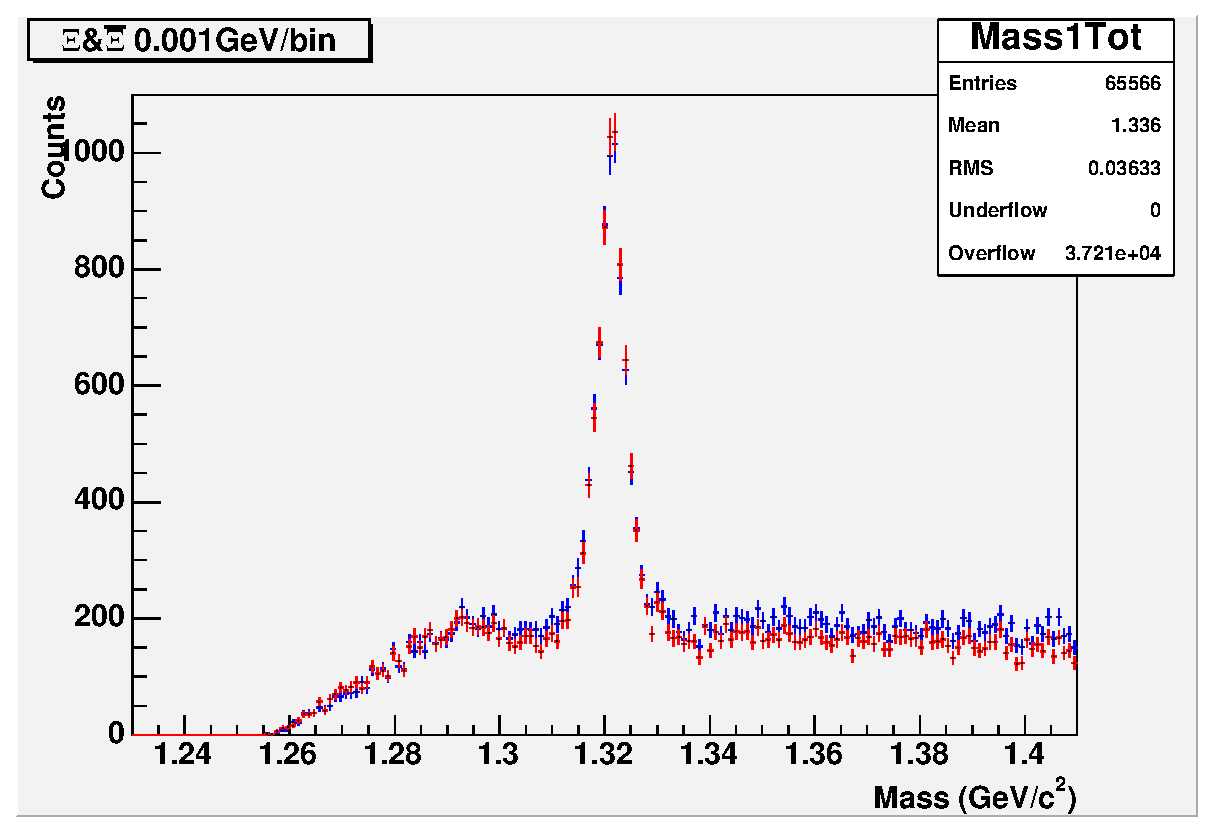
\epsfig{file=massCheck.eps,width=8cm} &
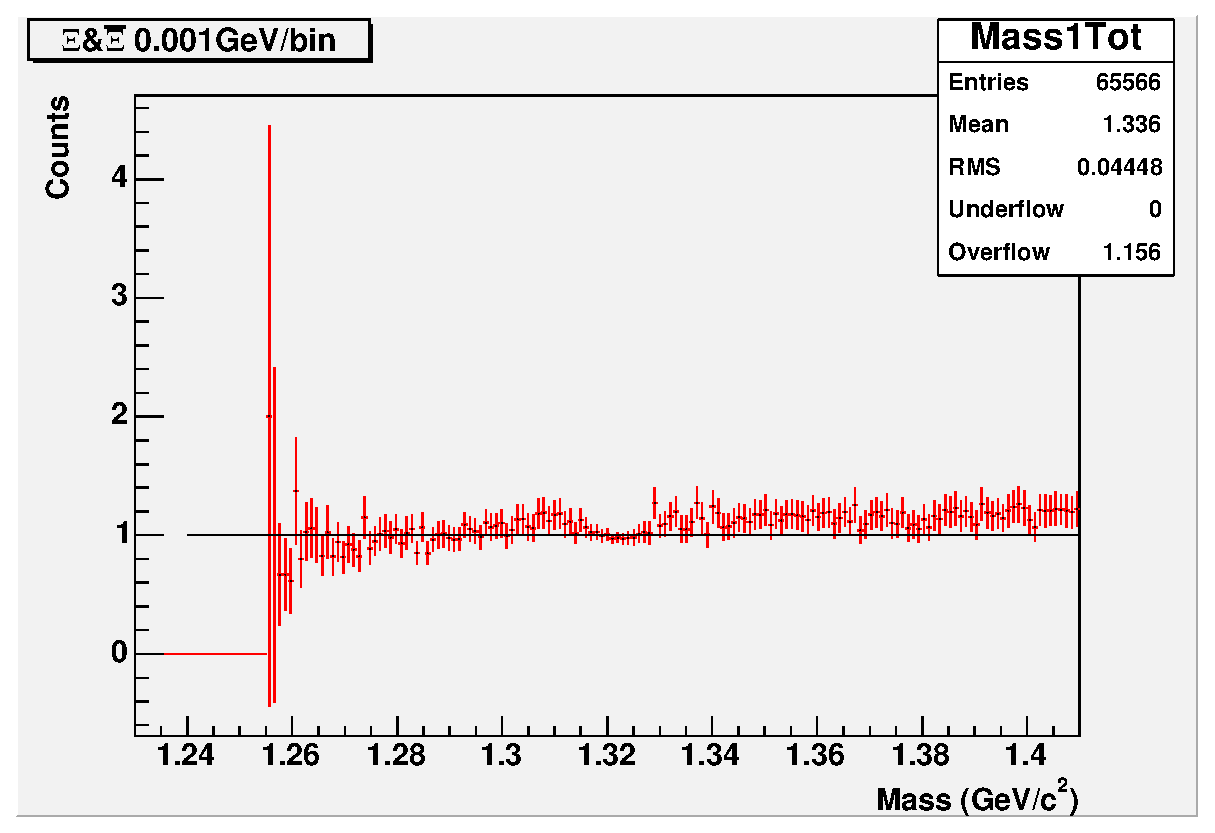
\epsfig{file=massRatio.eps,width=8cm} \\
\end{tabular}
\mycaptionBis{Comparison of the Fortran and C++ XiFinders}{Left plot : comparison of the XiFinders : Fortran invariant mass distribution in blue, C++ in red. Right plot~: ratio Fortran/C++}
\label{massCheck}
\end{center}

Details can be found here :\\
{\tt www.star.bnl.gov/protected/strange/faivre/utilities/xifindTest.html}


\subsection{Deep level tests}

Unlike the 2 other series, the first series of tests that I've made have been done only on the XiFinder (although I've made a V0Tester, but only to test the final variables and which V0's were found or not -- since the algorithm is different, deep level tests can't be made on the V0Finder). Furthermore, they test essentially... the background and not the signal, because of the so small number of signal Xi's ! (And technically~: it was run in the {\sc bfc}, so was very time- and disk-space-consuming, so only a few events could be processed). It consisted in printing the value of several or all the variables in the XiFinder algorithm, in Fortran and in C++, and comparing those values on a candidate-per-candidate basis.

Roughly speaking, I've printed 1/10th of the final results, and those forms a 3-cm high stack of paper sheets... So giving all the details is out of question ;-)

Since the Fortran maker and the C++ maker are run one after the other, the Xi vertices have to be identified. The event is identified by the position of the primary vertex, then the V0 is identified by the position of its vertex, and then the bachelor is identified with its momentum. This makes a unique Xi in Fortran and in C++. The codes that I've called ``testers" basically associate a Fortran Xi with the corresponding C++ Xi (if it exists), and then plot some distributions showing the differences. More details can be found in the talk that I gave during the strangeness workshop of November 2002 in {\sc ucla}, which can be found here~:\\
{\tt www.star.bnl.gov/protected/strange/faivre/talks/20021018/tlk2j2.html}

I've also inserted bugs on purpose and checked what was the effect on the output plots I was looking at~: the effect has been in all 4 cases immediately visible.

According to the type of the variables used, the error due to digitalisation and binary rounding of the floating-point numbers that we have to expect on the variables is~:
$$6.10^{-8} < \frac{\Delta x}{x} < 1.2\;10^{-7}$$

All 304 XiFinder variables have been checked, and the results are definitely satisfactory. The (very) few outliers were due to no value printed in the logfile, either in Fortran or in C++, for various reasons~; so they are not caused by a bug in the code.



\subsection{Global tests}

This series of tests consists in forgetting about the candidate-by-candidate comparisons, and checking that the distributions of various XiVertex variables ae similar between Fortran and C++, plus checking that the number of candidates found is the same. The tests are described here~:\\
{\tt www.star.bnl.gov/protected/strange/faivre/utilities/xifindTest.html}\\
and all the plots of the distributions can be seen on the same webpage.

Those tests show that the distributions and number of candidates found by the Fortran XiFinder and the C++ XiFinder are exactly similar when analysis cuts are applied, and almost exactly similar (see the webpage for details) when no cuts are applied~: the difference can't be seen with the eye, because it's almost always below 1 $\sigma$ of the statistical error bar.

Tests of the V0Finder show that some distributions are significantly different, but since the algorithm is different it's expected. The important thing is that when the invariant mass plots are compared once the analysis cuts are applied, no difference is seen in the number of signal found in the peak.









%\vspace{1cm}
\newpage

\section{To-do list}

There is no particular order and not everything is relevant/worth doing ;-)
\begin{maliste}
\item fabs vs TMath::Abs.
\item TThreeVector vs double[3].
\item Write more about tests in the documentation.
\item During the tests, I've seen that some tracks had all their parameters equal to 0~; I've set something in the code to prevent this (track is skipped, it avoids code crashing for dividing by 0 when inverting the curvature, for example), but haven't tried to understand why those tracks existed.
\item Fortran code doesn't treat correctly the cascade candidate when its V0 mass falls both in the $\Lambda$ and in the $\overline{\Lambda}$ mass hypothesis (it does only one of the 2 hypothesis). Influence on the tests ? (Concerns only a very small percentage of the candidates).
\item Bfield value is calculated from the momentum of the 1st track of the container, whatever its $p_\perp$~: could be useful to calculate Bfield only with a track that has a curvature reasonably high (i.e. not too high $p_\perp$).
\item Remove usage of {\tt xAns} and {\tt yAns} in {\tt StXiFinderMaker.cxx} : use directly {\tt xOut} and {\tt yOut}.
\item Flag $\chi^2_{Xi}$ negative even when the V0 is a Fortran one.
\item Change XiFinder algo : allow at most 1 stored Xi candidate per pair (V0,track). To choose~: take the intersection point that gives the smaller dca.
\item Etc...
\end{maliste}









%Essai avec Dav' de mettre une equation numerotee a gauche : pas moyen !! On dirait qu'on est obliges d'utiliser eqnaray pour numeroter une equation, et eqnarray centre systematiquement, quoi qu'on lui fasse. On ne peut meme pas l'utiliser dans un tableau ni dans une array. Pas plus que l'environnement equationarray (package eqnarray). La FAQ parle de la commande \lefteqn qui s'utilise avec eqnarray, mais sans expliquer comment elle marche. En mettant fleqn dans les options de documentclass, ca marche mais ca le fait pour toutes les equations du document (meme si on utilie \mathindent comme {\parindent blabla}).
%%$\begin{array}{cc}
%%a & b \\
%%c & d \\
%%\end{array}$
%%
%%
%%\begin{eqnarray}
%%a=b
%%\end{eqnarray}
%%
%%{%\mathindent=1cm
%%
%%
%%
%%\begin{eqnarray}
%%a=b
%%\end{eqnarray}
%%
%%}
%%
%%
%%\begin{eqnarray}
%%a=b
%%\end{eqnarray}
%%
%%
%%\begin{flushleft}
%%$\begin{array}{c}
%%x=y
%%\end{array}$
%%\end{flushleft}
%%
%%Ici c'est moi.
%%
%%\lefteqn{
%%\begin{eqnarray}
%%a = b
%%\end{eqnarray}}
%
%\begin{eqnarray}
%x=y
%\end{eqnarray}
%
%\hspace{50pt}
%\begin{eqnarray}
%a=b
%\end{eqnarray}
%
%
%%\begin{flushleft}
%%\hspace{50pt}
%%\begin{alignat}{1}
%%a = b \\
%%c = d
%%\end{alignat}
%%\end{flushleft}
%
%%$\begin{array}{l}
%%\begin{array}{c}
%%$$x=y$$
%%\end{array} \\ 
%%\begin{array}{c}
%%q=y
%%\end{array}
%%
%%\end{array}$
%
%
%\parbox{2cm}{
%\begin{eqnarray}
%%x = y \hfill a \\
%x = y \hspace{12cm} ~
%\end{eqnarray}
%}









\end{document}







